\documentclass[runningheads]{llncs}
%
\usepackage{graphicx}
% Used for displaying a sample figure. If possible, figure files should
% be included in EPS format.
%
% If you use the hyperref package, please uncomment the following line
% to display URLs in blue roman font according to Springer's eBook style:
% \renewcommand\UrlFont{\color{blue}\rmfamily}

\usepackage{enumitem}
\usepackage{amsmath}
\usepackage{amsfonts}
\usepackage{graphics}
\usepackage{multirow}
\usepackage{floatrow}

\begin{document}
%
\title{The Standard Capacity Model: \\Towards a Polyhedron Representation of\\ Container Vessel Capacity\thanks{This research is supported by the Danish Maritime Fund grant no. 2016-064.}}
%
\titlerunning{The Standard Capacity Model}
% If the paper title is too long for the running head, you can set
% an abbreviated paper title here
%
\author{Mai Lise Ajspur\inst{1} \and
Rune M{\o}ller Jensen\inst{1}}
%
%\email{ajspur,rmj@itu.dk}

\authorrunning{M.L. Ajspur and R.M. Jensen}
% First names are abbreviated in the running head.
% If there are more than two authors, 'et al.' is used.
%
\institute{The IT University of Copenhagen, Rued Langaards Vej 7, 2300 Copeenhagen S, Denmark}
%
\maketitle              % typeset the header of the contribution
%
\begin{abstract}
The abstract should briefly summarize the contents of the paper in
15--250 words.

\keywords{First keyword  \and Second keyword \and Another keyword.}
\end{abstract}

\section{Introduction}
Container liner shipping is a major driver of the world economy \cite{TE13}. There are more than 5000 container vessels in the world today \cite{RMT16}, mostly sailing on cyclic services with published fixed weekly schedules and freight rates. Liner shipping companies adjust their service networks and fleet over the year to fit seasonal trends and long-term developments in the world economy, but they seldom make fleet and network changes due to current cargo on the network and known bookings (Mikkel persal communic). For that reason, it is a central business objective to maximize the utilization of the service network. Any free capacity in the network is an opportunity for business.

In this aspect, the container shipping and airline industry is similar. It is all about filling the slots on the vessels. A closer inspection shows, however, that the domains are rather different. Air planes are usually completely emptied at each destination, and an empty seat in most cases means that the plane can fit one more passenger. This has enabled the airlines to apply advanced revenue management methods such as dynamic pricing and over-booking to maximize the utilization of the planes.

Previous work has studied how to apply revenue management methods in the liner shipping industry (e.g., Sebastian), but it has turned out to be challenging in practice. A major obstacle is how to compute the free capacity of a container vessel. It is not simply the number of vacant slots on the vessel. A large number of local and global constraints may cause slots to be impossible to use including: stacking limitations due to different length, height, power need (reefer containers), and dangerous content of containers; limited volume, weight, and securing capacity of container stacks; vessel hydrostatics like stability requirements and stress force limitations; containers blocking each other due to different port of discharge; capacity preserving stowage patterns; and work balancing of quay cranes (see Section~\ref{} for details).

It is recognized by leading economists that this problem blocks a paradigm change in liner shipping. According to Martin Stopford the ability to match spare capacity to cargo in need of transportation on the fly would allow the "Uberisation" of the freight business \cite{EApril18}. Today, the higher sales and cargo flow functions in liner shipping companies are unable to make these matchings. The spare capacity of a container vessel is often simply calculated as its maximum volume, weight, and reefer container capacity subtracted the capacity taken up by on board cargo without consideration of losses due stowage restrictions and rules (personal communication Mikkel M). This can cause great over-estimates of the free capacity of the vessels (delgado thesis).

In the last two decades, a number of automated stowage planning methods have been published (e.g., roach, kim kang, ambrosino, pacino (ICLL 11, all late publications). The input to these methods is the arrival condition of the vessel and a list of containers to load and the output is a stowage plan. As such, these methods are unable to compute the spare capacity of the vessel, since the containers to load are assumed to be known. Several of the contributions, though, apply optimization models, where the containers to load can act as decision variables rather than constants (e.g. ambrosino Aberlto pacino, etc). There is also recent work on maximizing the utilization of a vessel on a given circular service route with limitations on expected cargo (alberto, pacino). 

These models can be used to compute the spare capacity of a vessel. In practice, though, they can be challenging to apply in higher functions such as sales and cargo flow. The stowage planning problem is NP-hard (org. NP hardness proof), even in its various abstract versions (our NP-hardness proof). This means that the stowage optimization models can take long time to solve, which also happens in practice (e.g., pacino 11). Since it can take more than five hours to generate a stowage plan manually, this is an acceptable evil in stowage planning. In higher functions, on the other hand, capacity models can be parts of larger optimization models which require that they are scalable. For instance, in capacity and uptake management, a cargo flow network could be used to match cargo demand with spare capacity. In such a network over a handful of weeks of a major trade line, there would be thousands of edges representing voyage legs, and each of these would be associated with a capacity model. 

To address this challenge, this paper introduces the {\em standard capacity model} (SCM). The SCM is based on several insights from our previous work on stowage planning optimization. First, a lot of the complexity and inaccessibility of these models stem from the fact that data describing container vessels is spatially misaligned. To clear this, the SVCM interpolates vessel data to align with the endpoints of each bay. Second, stowage optimization models have many details that can be abstracted away in capacity calculations. To this end, the granularity of SCMs can be adjusted. At the finest level, each bay form a {\em section}. At coarser levels, adjacent sections are merged. Third but not least, our previous studies of vessel hydrostatics (cite ICCL on hydro model) show that these can be accurately approximated by linear functions within a displacement interval. The intractable elements of stowage planning include separation rules of containers with dangerous goods and the fact that quay cranes only can discharge containers from the top of stacks (org. NP hardness proof). In more abstract capacity models, though, it may be possible to express some of these combinatorial aspects as linear trade-offs. In particular, a significant body of industrial R\&D shows that surprisingly many highly complex aspects of stowage planning such as the limited forces in lashing gear either can be linearly expressed or can be approximated with convex step-wise linear functions (cite optivation). Our objective is in time to mature SCM with these advanced linear models. Moreover, in this paper we introduce to our knowledge, the first linear approximation of hydrostatic equilibrium and metacentric height that is independent of vessel displacement. The ultimate goal of SVCM is to provide an accurate and compact polyhedron (i.e., LP) model of vessel capacity to e.g. intregrate in large cargo flow networks for uptake and capacity management optimization.

Our results show ...

The remainder of this paper is organized as follows. ...

\section{Problem Formulation}

Container vessels mainly transport ISO containers with the dominating lengths 20', 40', and 45'. The containers are usually 8' wide. There are two common heights: standard 8'6" (DC) and high-cube 9'6" (HC). Containers have corner fittings that allow them to be stacked about 10 high. 45DC and 20HC are rare. {\em Reefer} containers are refrigerated and need external power. {\em Out-of-gauge} (OOG) containers have irregular dimensions (e.g., open top containers with cargo sticking up). Flatracks are flat containers to carry non-containerized cargo (break-bulk). {\em DG} containers contain dangerous goods such as fireworks and chemicals. They must be placed according to complex separation rules and may not be allowed near reefers since these are spark generators. 

As shown in Fig.~\ref{fig:vessel}, the cargo space of a container vessel is divided into {\em bays}. A bay consist of stacks (rows) of cells. A cell is divided into a fore and aft \emph{slot} and can accordingly hold one 40' (or 45') container or two 20' containers. Some cells have power plugs allowing reefers to be stowed. Each bay is divided into stowage areas above and under {\em hatch covers} that separate on deck and below deck cells. A vessel has a cargo securing manual that details how the vessel can be stowed securely.    
\begin{figure}[h!]
	\centering
		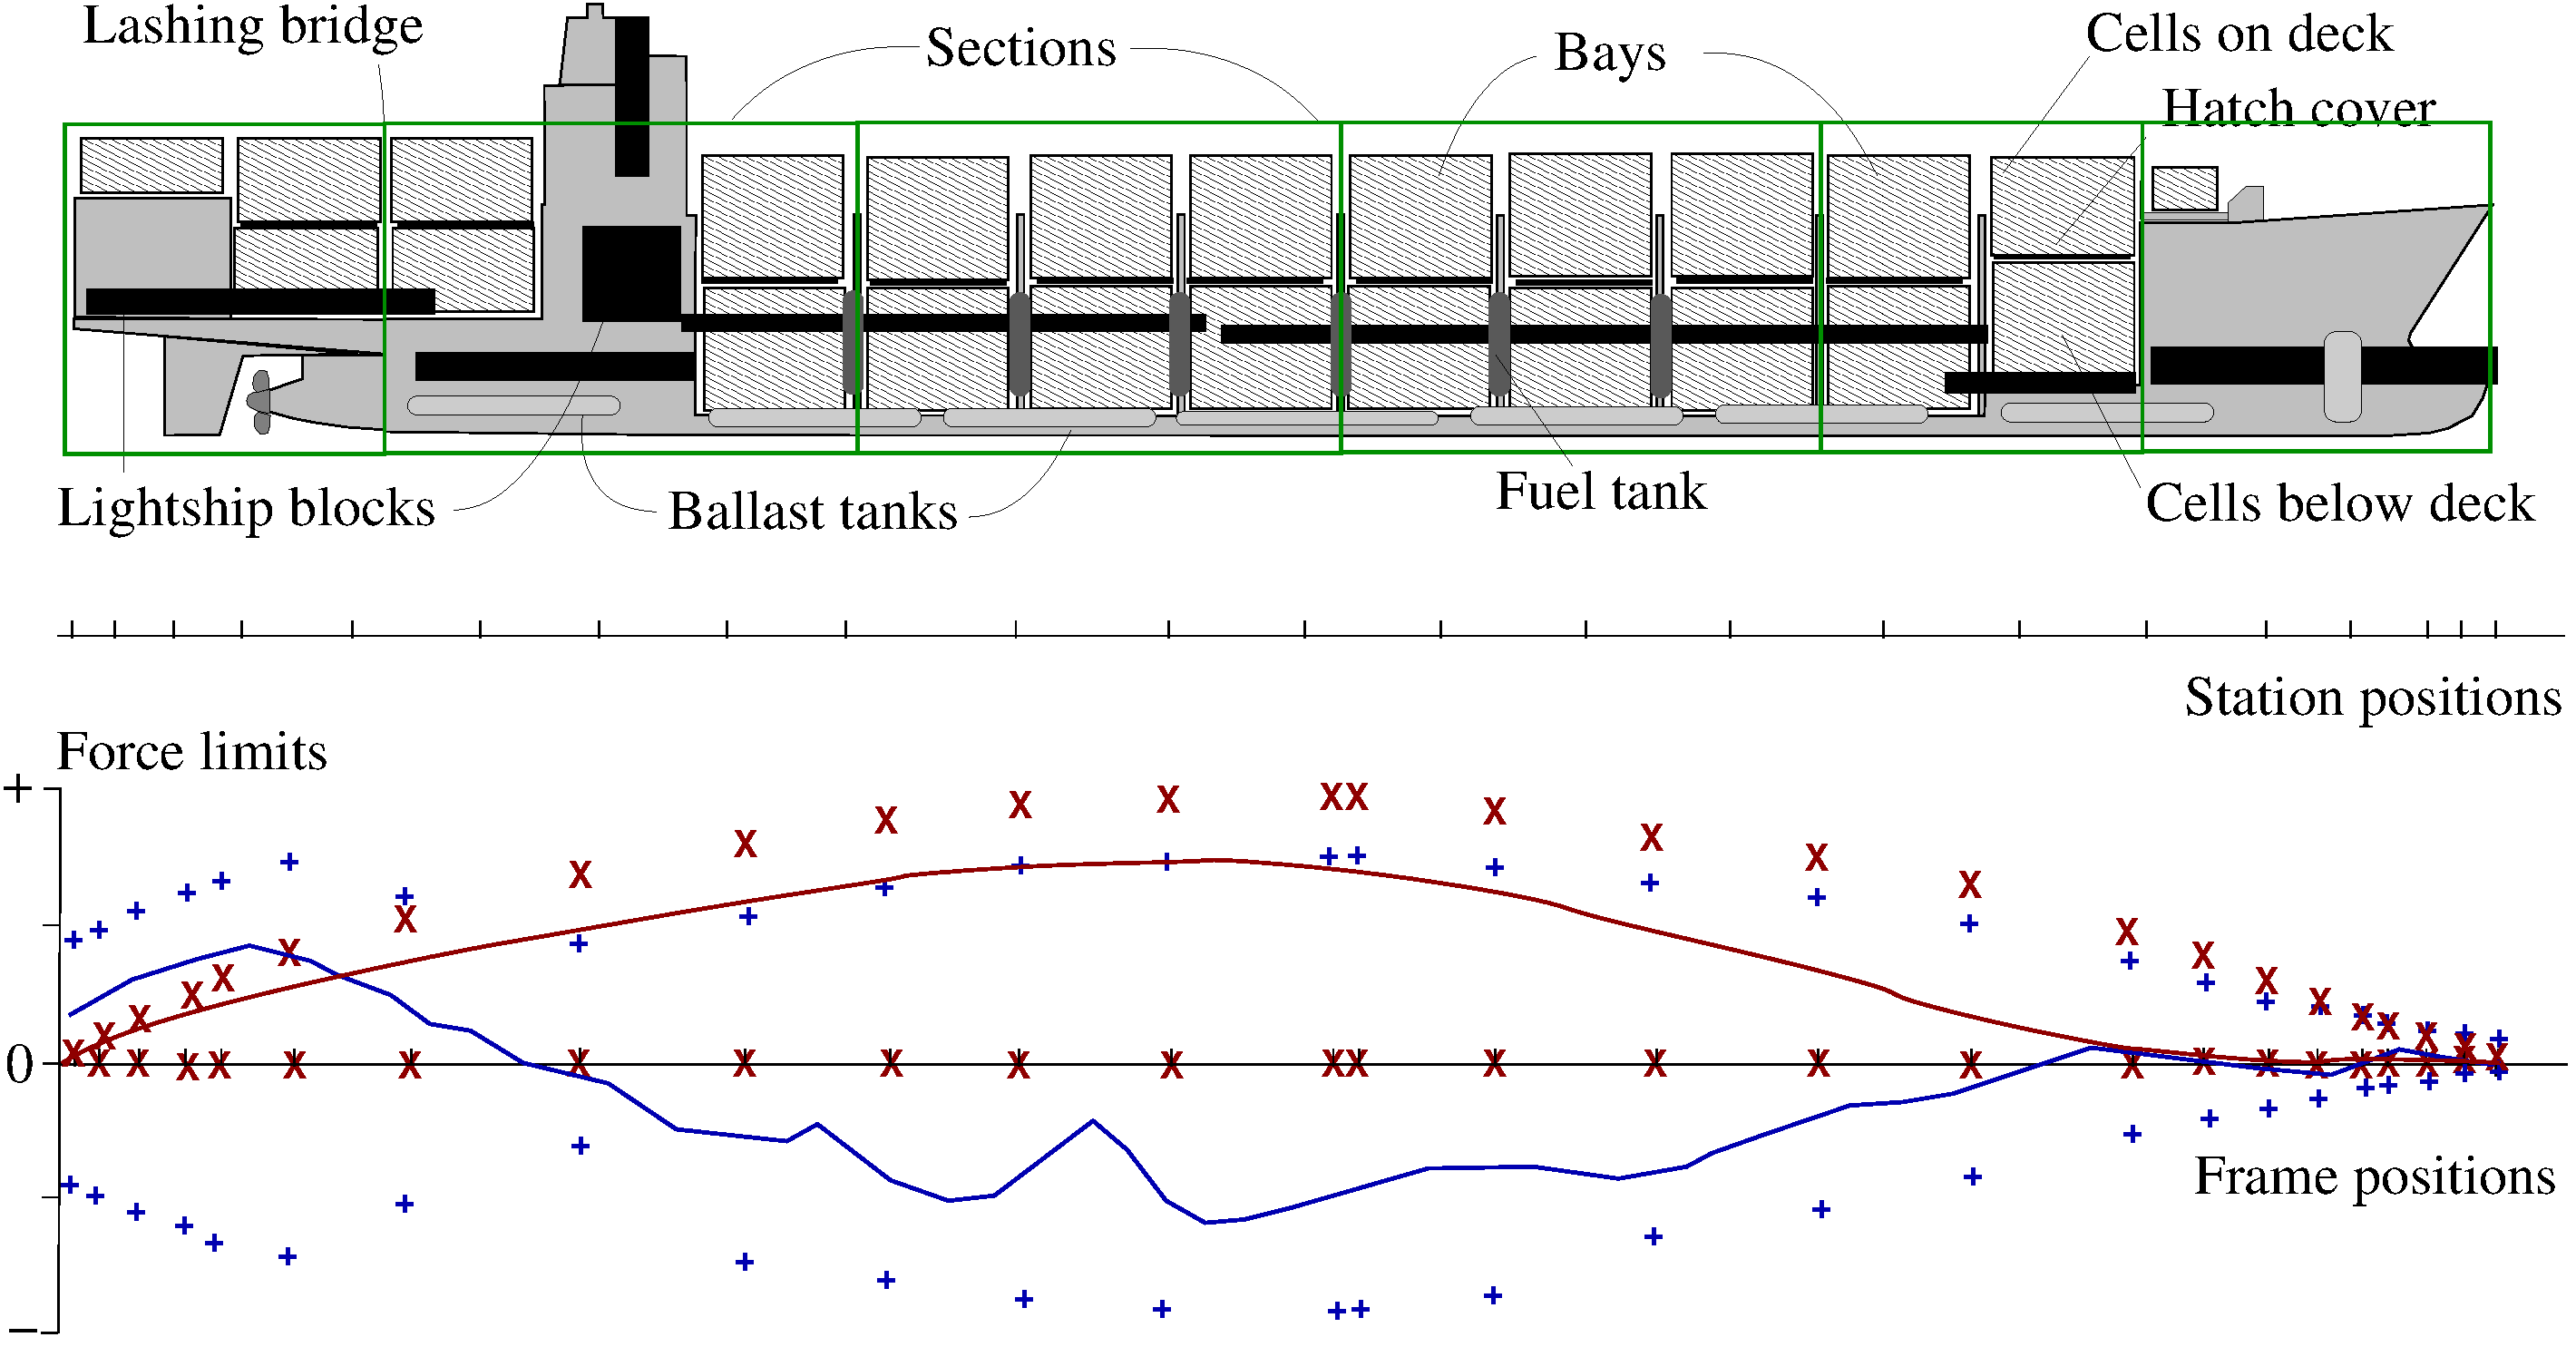
\includegraphics[scale=0.24]{figures/vesselAndForces.pdf}
	\caption{Top: the structure of a cellular container vessel and an example of a section partitioning that can be used by the standard capacity model. Bottom: an example of the shear forces (blue curve) and bending moments (red curve) along a vessel. Blue plus signs and red crosses are the associated force limits given by the classification society for a set of frame positions.} 
	\label{fig:vessel}
\end{figure}

The precise position of bays, fuel tanks and ballast water tanks are provided by the shipyard that build the vessel. The yard also provides details about the {\em lightship}, which is the vessel without cargo, fuel or ballast water. This information can be given as a set of blocks with known mass and center of gravity as shown in Fig.~\ref{fig:vessel}.
From this data, the resulting center of gravity of the vessel can be calculated. 

The Bonjean table of the vessel can be used to compute its center of buoyancy. For a set of cross-section {\em stations} along the vessel, it gives the submerged area as a function of the distance from the keel to the water line ({\em draft}) of the station. A vessel is in hydrostatic equilibrium when the center of buoyancy and gravity are vertically aligned. In this condition, the vessel floats at rest in the water at a stable draft, {\em trim}, and {\em list}. Trim is the difference between aft and fore draft of the vessel (i.e., nose up is positive trim). The total weight of a vessel is referred to as its {\em displacement} and has different summer and winter limits depending on sea location. Many ports such as Hamburg have significant tide dependent draft limits. Pilots usually require that the vessel is at even keel (i.e., trim zero) during their operation. At any trim, {\em line-of-sight} (LOS) rules require that objects on the surface can be seen from the bridge until 500 meters in front of the vessel. Fuel efficient trims are typically around -2 meters (i.e., nose down). The list is the heeling angle. The list should be near zero to preserve transversal stability. 

While the sum of buoyancy and gravity forces are vertically aligned at hydrostatic equilibrium, the forces acting on the vessel are usually distributed unevenly over the hull.
\begin{figure}[h!]
	\centering
		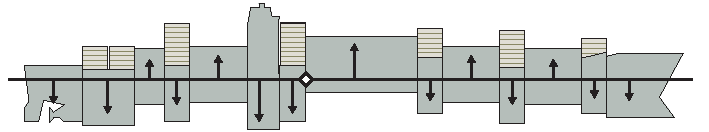
\includegraphics[scale=1]{figures/3_12.pdf}
	\caption{An example of the resulting gravity and buoyancy forces (black arrows) acting in the longitudinal direction at hydrostatic equilibrium.}
	\label{fig:forces}
\end{figure}
Fig.~\ref{fig:forces} shows an example of the resulting gravity and buoyancy forces and how they would cause sections of the vessel to change draft (and list) if they could move freely. The counteracting forces in the hull that prevents such movement are referred to as {\em stress forces}. The critical stress forces acting on a vessel are {\em shear forces} (SF), {\em bending moments} (BM), and {\em torsion moments} (TM). These forces are defined relative to a cross-section of the vessel. Consider the cross section indicated by the white diamond in Fig.~\ref{fig:forces}. SF in the cross section is the sum of forces fore of the cross section.~\footnote{SF can just as well be defined as the sum forces aft of the cross section. The reason is that since the vessel is at hydrostatic equilibrium, the two forces must be equal but with opposite sign.} BM is the sum of forces each multiplied with the longitudinal distance to them. TM is caused by the distribution of forces over the center line. It is defined like BM using the transversal distance to the force. SF and BM measure how much the forces try to shear and bend the cross section, while TM measures how much they try to twist it. The classification society of the vessel defines minimum and maximum limits of these forces for a number of frame positions along the vessel. Fig.~\ref{fig:vessel} shows an example of SF and BM forces. Notice that frame and station positions are misaligned. A ship typically has higher gravity forces than buoyancy forces in the bow and stern. Consequently, SF forces are positive aft and negative fore while BM is high midship. TM  limits can be critical on modern vessels due to their extended width.

The transversal stability of a vessel mainly depends on the width of the vessel and how high the center of gravity is over the keel.  When the vessel lists due to an external force, the center of buoyancy moves transversally in the direction of the list. If the vertical center of gravity is high, it may move faster in the direction of list causing the vessel to capsize. Transversal stability is expressed in {\em metacentric height} and must be above a given minimum.  

\section{The Standard Capacity Model}

The purpose of the Standard Capacity Model (SCM) is to
\begin{enumerate}
\item simplify the data representation of vessels by aligning all data points to a reference system defined by sections,
\item simplify the capacity constraints of vessels by a linear polyhedron approximation,
\item provide a model with an adjustable level of detail.  
\end{enumerate}

As mentioned in the introduction, the key idea of SCM is to partition the vessel into sections that are aligned with bays. At the finest level of detail, sections hold at most one bay. At coarser levels, some sections are merged. As an example, Fig.~\ref{fig:vessel} shows a partitioning of a vessel into six sections, where the largest sections aggregate three bays. The choice of sections depends on the application. For large cargo flow models, it may only be computationally tractable with a few sections per vessel. The choice also depends on the cellular structure of the vessel. A section partitioning also should be made with stowage trade-offs in mind (e.g., cluster bays bays with same reefer plug and lashing bridge arrangement).

This paper focuses on the main building block of SCM which, to our knowledge, is the first linear approximation to a hydrostatic model of a container vessel that allows variable displacement. We model the hydrostatic equilibrium of forces acting on the vessel in the longitudinal direction. This enables SCM to model core parameters such as draft, trim, BM and SF and the approach is possible to extend in the transversal and vertical direction to model list, TM, and metacentric height. For this purpose, we need to approximate the relations between the variables of SCM (see Table~\ref{tab:variables}) as linear equations
  
The mass of a section is the sum of masses of lightship blocks, ballast water, fuel, and cargo within the boundaries of the section. If a block (e.g., a ballast water tank) extends beyond the section, only the mass of the fraction within the section is included in the sum. If we assume that all gravity forces act from the longitudinal mid-point of the section, the resulting gravity force clearly can expressed as a linear function of the cargo and ballast water in the section.~\footnote{In future versions of SCM, this point may be divided in the transversal and vertical direction to estimate TM and metacentric height .}    

The buoyancy of a section depends on the draft of the section rather than its weight. It can be estimated from the Bonjean table of the vessel. Recall that the Bonjean table for each station gives the submerged area of a cross section at the station as a function of the mid-ship draft at even keel. Fig~\ref{fig:Bonjean} shows the Bonjean data of a 15000 TEU container vessel with a representative fine form hull. Notice that the curves are shown over the complete operational draft range of the vessel. The lightship draft is about four meters and the maximum summer draft is about 16 meters.
\begin{figure}[h!]
  \begin{tabular}{ccc}
 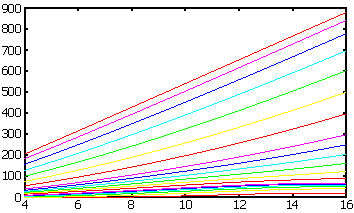
\includegraphics[scale=0.14]{figures/BonjeanFore} &  &   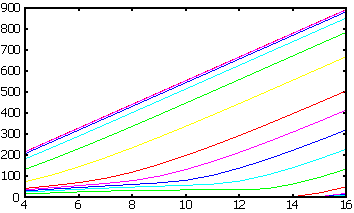
\includegraphics[scale=0.14]{figures/BonjeanAft} \\
          (a)                              &  &                   (b)   \\
 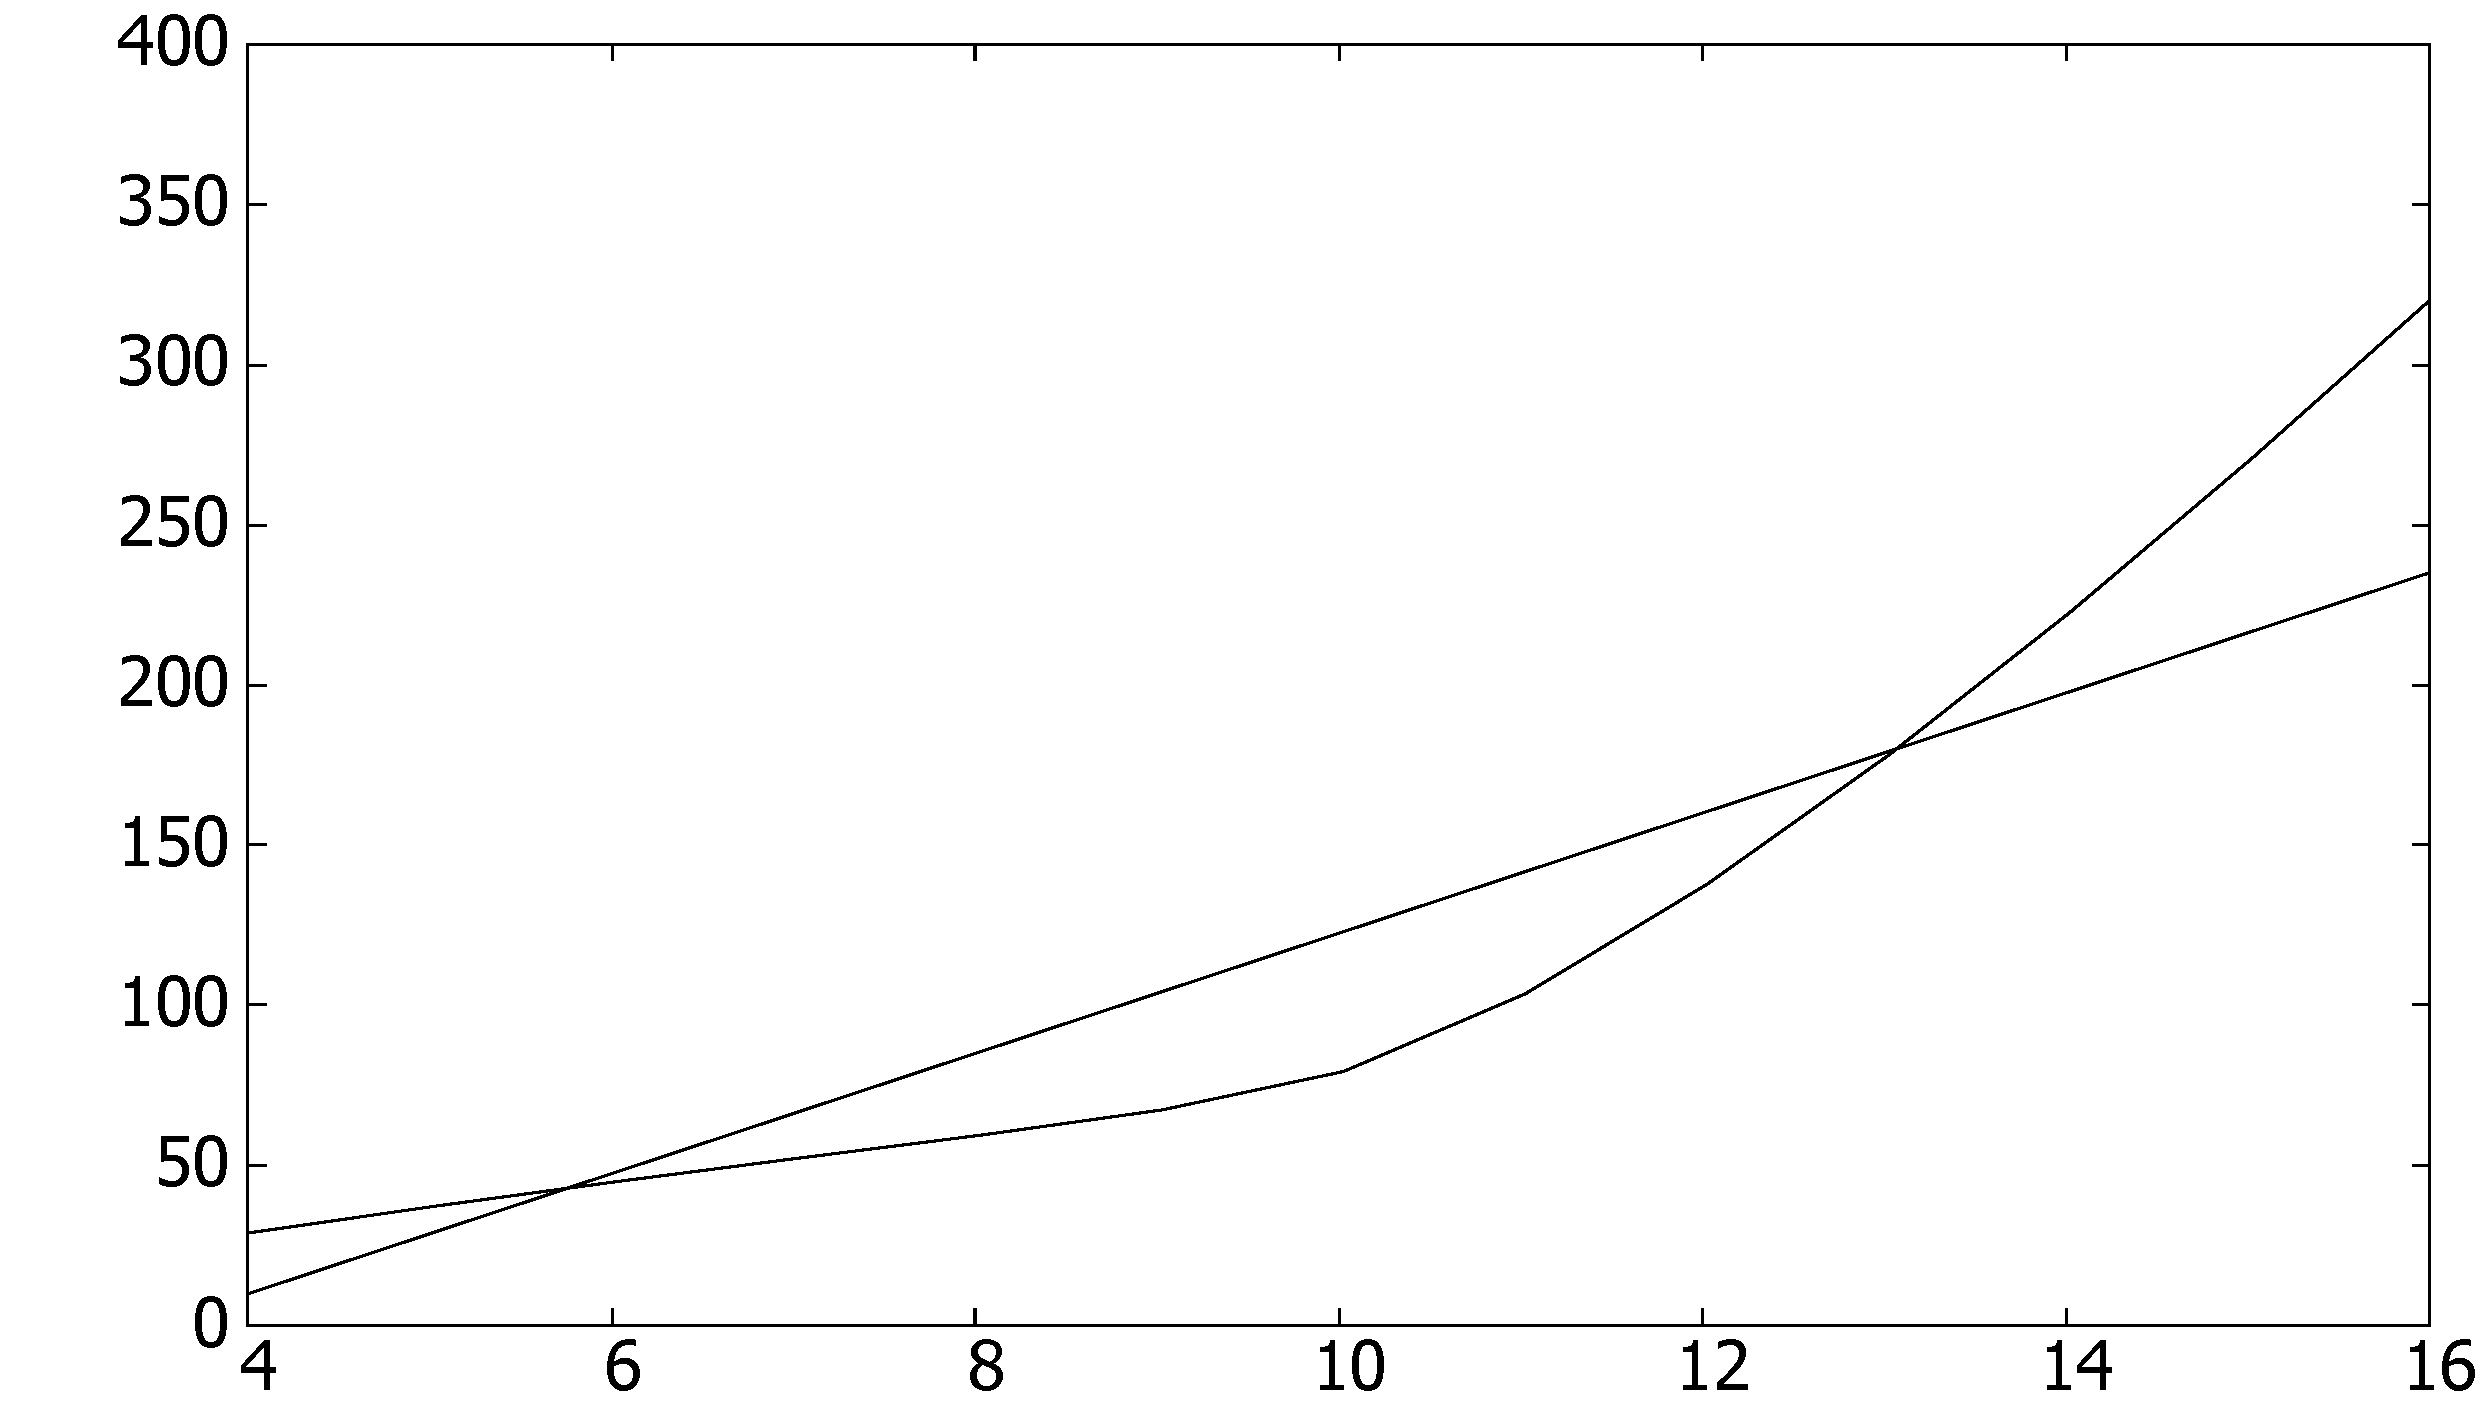
\includegraphics[scale=0.14]{figures/BonjeanLinear1} &  &   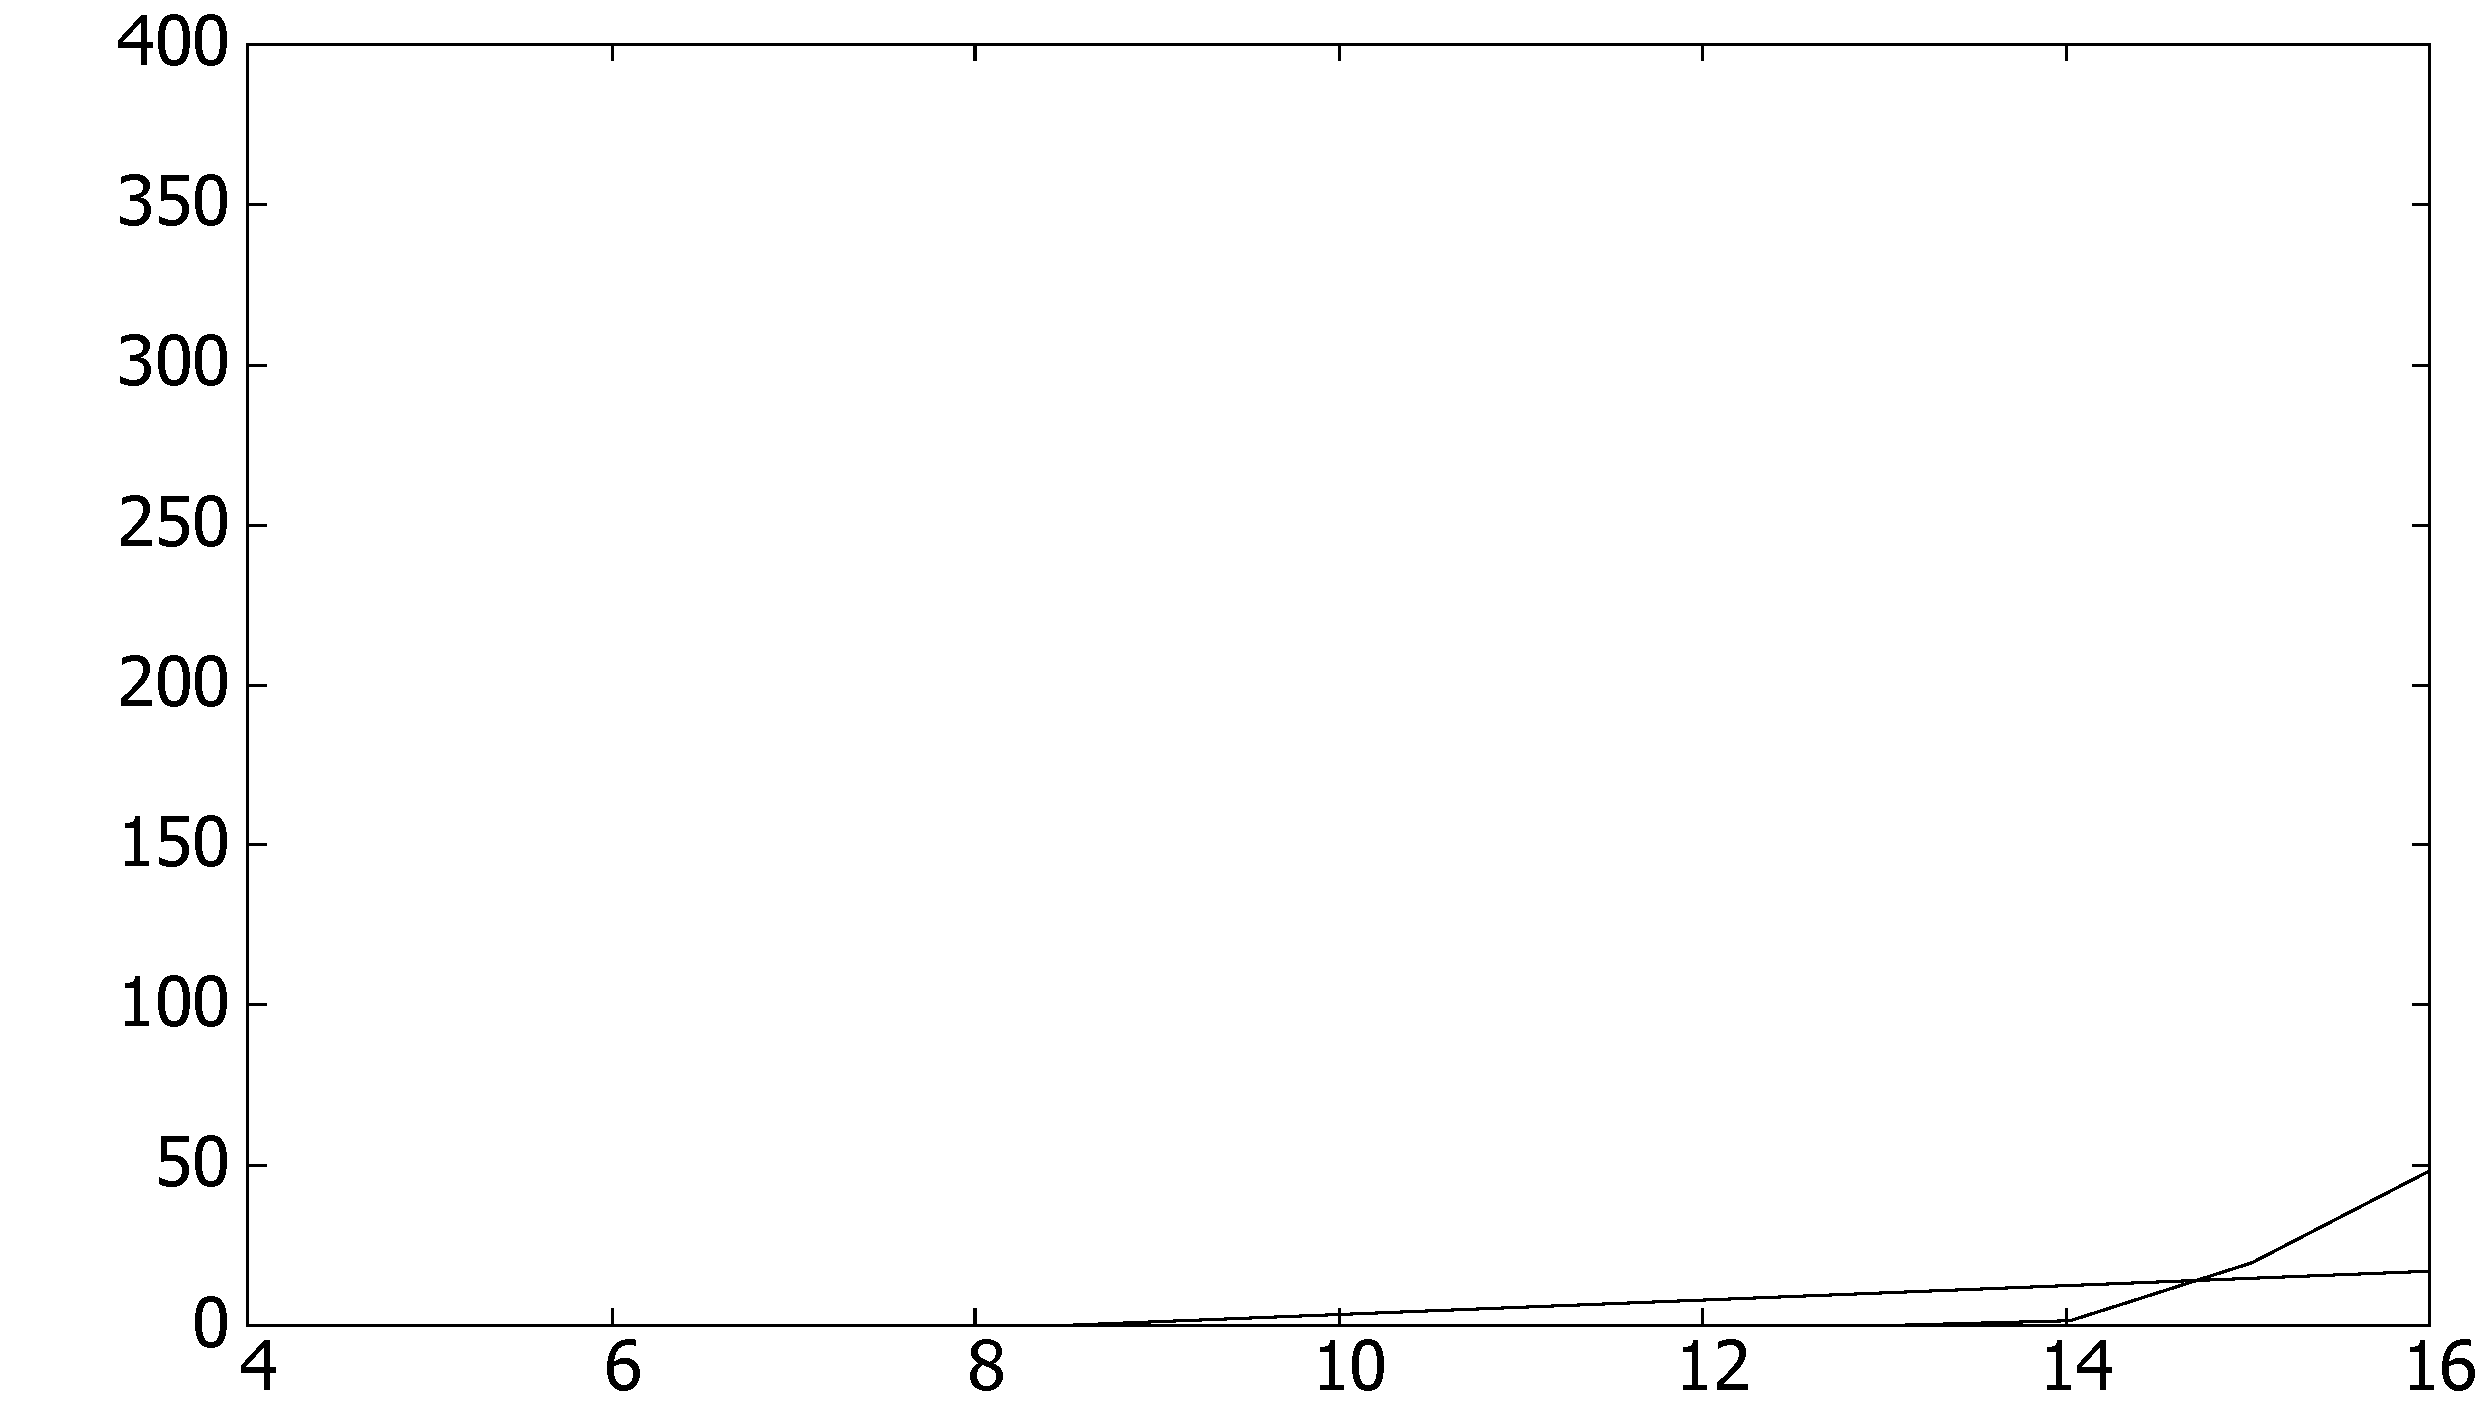
\includegraphics[scale=0.14]{figures/BonjeanLinear2} \\
          (c)                              &  &                   (d)   
  \end{tabular}
  \caption{Subermged area of fore (a) and aft (b) stations as a function of mid-ship draft at even keel.}\label{fig:Bonjean}
\end{figure}

The mid-ship stations (top curves in graph (a) and (b)) have the largest submerged areas. Since the vessel has vertical sides at drafts above four meters in this part, the submerged areas grow linearly with the draft from this level. The curves for fore sections are slightly non-linear, while they for the aft sections (lower curves graph (b)) are significantly non-linear. The reason is that the full stern only touches the water at maximum draft. 

Despite these non-linearities, the dominating shape of the vessel is box-formed with vertical sides within the operational draft area. This means that the horizontal surface formed by the water line approximately has fixed shape such that the longitudinal moment needed to achieve a particular trim adjustment (say plus one meter) is constant for different displacements. This conclusion seems in conflict with previously published data shown in Fig.~\ref{fig:hdtrim}. The graph shows trim as a function of displacement (i.e., draft) and longitudinal center of gravity (lcg) for the same vessel. For a fixed lcg (i.e., fixed longitudinal moment) this graph shows a highly non-linear relation between trim and displacement. A closer inspection of the graph, however, reveals that the displacement range is far out of operational levels which are above a fuelled ship of about 75K tons and below maximum summer displacement of 218K tons. Between 100K and 218K, we do see a rather linear relation between trim and displacement as expected from the analysis above.  

\begin{figure}[h!]
\begin{center}
  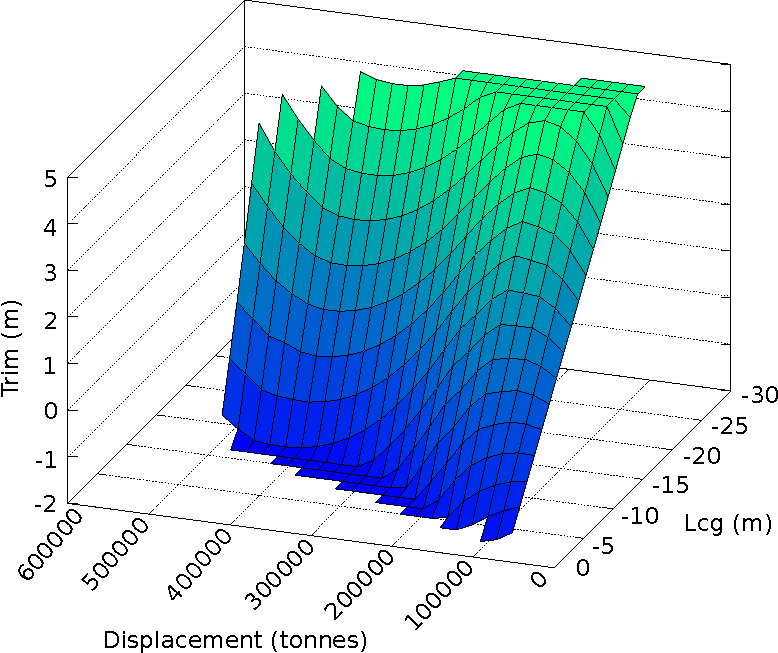
\includegraphics[scale=0.5]{figures/hd_trim}
\end{center}
\caption{Trim as a function of displacement and lcg (CITE Alberto).}
\label{fig:hdtrim}
\end{figure}


Due to this, we approximate the vessel as box formed sections. To this end, SCM uses a linear approximation to all Bonjean curves. Two examples of the linearisations of aft curves are shown in Fig.~\ref{fig:Bonjean}(a,b). Assume that the two boundaries of section $k$ lie between station $i$ and $i+1$ and $j-1$ and $j$, respectively, as shown in Fig.~\ref{fig:Bapprox} . Further assume that the submerged area of station $s$ is $A_s$ according to the linearisation above. We then have that the buoyancy of section $k$ in tons is 
\begin{equation}
\frac{d}{2} \sum_{s=i}^{j-1} f_s l_s (A_{s+1} + A_{s}), \label{eq:area}    
\end{equation}
where $d$ is the density of salt water, $f_s$ is the longitudinal fraction of station $s$ to $s+1$ within the boundary of section $k$  
of the vessel spans station $i$ to $j$, and $l_s$ is the distance between the two stations.
\begin{figure}[h!]
\begin{center}
  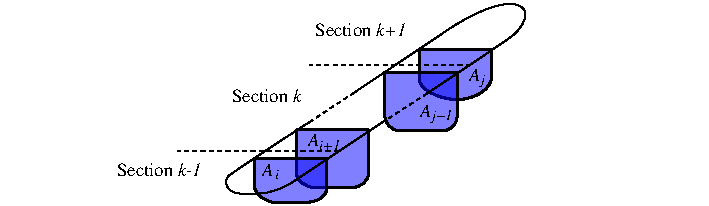
\includegraphics[scale=0.5]{figures/BouyancyApprox}
\end{center}
\caption{Bouyancy approximation of a section.}
\label{fig:Bapprox}
\end{figure}

At maximum summer displacement of the example vessel, this approximation underestimates the buoyancy with about $3.06\%$. This is probably due to the slight convex shape of the hull. Consequently we adjust the linearization such that it predicts the correct summer displacement. 

Below we present SCM as an LP feasible set (i.e., a polyhedron). Table~\ref{tab:setsconstants} and \ref{tab:variables} contain the explanation of symbols for sets, constants, and variables used in the model. 

\begin{table}[h!]
\begin{center}
\begin{tabular}{rl}
    & \textbf{\textit{Sets}}\\
    $\mathcal{S}$ & Sections.\\
    $\mathcal{T}$ & Container types. \\
    & \\
    & \textbf{\textit{Constants}}\\
    $L_s$         & Length of section $s$ in meters.\\
    $W^0_s$       & Lightship weight of section $s$ in tons.\\
    $\mathrm{SF}^{+/-}_s$ & Positive and negative shear force limit in tons.\\ 
    $\mathrm{BM}^{+/-}_s$ & Positive and negative bending moment limit in tons meters.\\ 
    $W_s$         & Container weight capacity of section $s$ in tons.\\
    $V_s$         & Container volume capacity of section $s$ in TEU.\\
    $R_s$         & Number of reefer plugs in section $s$.\\ 
    $\Phi_s,\Psi_s,\Theta_s$ & Buoyancy linearisation constants of section $s$.\\        
    $W_\tau$      & Weight of container type $\tau$.\\
    $V_\tau$      & Volume of container type $\tau$ in TEU.\\
    $R_\tau$      & Indicates whether container type $\tau$ is reefer.\\
\end{tabular}
\end{center}
\caption{Sets and constants used in SCM.}
\label{tab:setsconstants}
\end{table}

Sections are numbered from the bow (i.e., $\mathcal{S} = \{ 1,2,\ldots \}$. They form a complete physical partitioning of the vessel such that all of its parts belong to a section and no part belong to two sections. Section borders are aligned with bays. A section can not divide a bay. An example of a section partitioning with six sections is shown with green boxes in Fig~\ref{fig:vessel}. Let $L^G_s = \sum_{s'>s} L_{s'} + L_s / 2$ denote the distance from the stern to the center of gravity (mid-point) of section $s$. Further, let $L^F_s = \sum_{s' \geq s} L_{s'}$ denote the fore boundary of section $s$ (reference point for stress forces).

A container type $\tau \in \mathcal{T}$ is a triple $(l,r,w)$, where $l \in \{20,40,45\}$ is the length of the container, $r \in \{ \mathit{RF},\mathit{NR} \}$ is the reefer properties of the container (reefer or non-reefer), $w \in \{9,14,29\}$ is the weight class of the container expressed as the average weight of containers in the class in metric tons. The buoyancy linearisation constants $\Phi^B_s,\Psi^B_s$ of section $s$ are approximated from equation~\ref{eq:area}.


\begin{table} [!ht]
\begin{center}
\begin{tabular}{rl}
    & \textbf{\textit{Variables}}\\
    $w$             & Weight (i.e. displacement) of the vessel in tons.\\
    $d$             & Draft aft in meters at the stern of the vessel.\\
    $\mathit{tr}$   & Trim of the vessel in meters.\\
    $w_s$           & Weight of section $s$ in meters.\\
    $b_s$           & Buoyancy of section $s$ in meters.\\
    $r_s$           & Resulting force acting on section $s$ in tons.\\
    $\mathit{sf}_s$ & Shear force between section $s$ and $s+1$ in tons. \\
    $\mathit{bm}_s$ & Bending moment between section $s$ and $s+1$ in tons meters. \\
    $t_s$           & Weight of tank content of section $s$ in meters.\\ 
    $c^\tau_s$      & Number of containers of type $\tau$ in section $s$.
\end{tabular}
\end{center}
\caption{Variables used in SCM.}
\label{tab:variables}
\end{table}

The domain of all variables is $\mathbb{R}^+_0$. In particular, this means that we relax the integrality of $c^\tau_s$. Due to the large number containers in each bay (near 1000 in average on modern vessels), previous work shows negligible impact of this relaxation in practice (CITE Dario). Also notice that none of the variables are identified as decision variables. This is on purpose since any subset of the variables can act as decision variables depending on the application of SCM.

SCM is a polyhedron over the variables defined by the following linear equations and inequalities. 
\begin{alignat}{15}    
                & b_s = \Phi_s d + \Psi_s \mathit{tr} + \Theta_s && \forall s \in \mathcal{S}  \label{eq:constr2}\\
                & w_s = W^0_s + t_s + \sum_{\tau \in \mathcal{T}} W_\tau c^\tau_s \hspace{5mm} && \forall s \in \mathcal{S}  \label{eq:constr3}\\
                & r_s = b_s - w_s  \label{eq:constr4}\\                
                & w = \sum_{s \in \mathcal{S}} w_s &&   \label{eq:constr5}\\
                & w = \sum_{s \in \mathcal{S}} b_s &&   \label{eq:constr6}\\
                & 0 = \sum_{s \in \mathcal{S}} L^G_s r_s &&   \label{eq:constr7}\\
                & \mathit{sf}_s = \sum_{s' < s} r_{s'} &&  \forall s \in \mathcal{S} \setminus \{1\}  \label{eq:constr8}\\                      
                & \mathit{bm}_s = \sum_{s' < s} (L^G_{s'} - L^F_s) r_s' &&  \forall s \in \mathcal{S} \setminus \{1\}  \label{eq:constr9}\\                      
                & \mathrm{SF}^-_s \leq \mathit{sf}_s \leq \mathrm{SF}^+_s      &&  \forall s \in \mathcal{S} \setminus \{1\}  \label{eq:constrA}\\           
                & \mathrm{BM}^-_s \leq \mathit{bm}_s \leq \mathrm{BM}^+_s      &&  \forall s \in \mathcal{S} \setminus \{1\}  \label{eq:constrB}\\           
                & \sum_{\tau \in \mathcal{T}} W_\tau c^\tau_s \leq W_s &&  \forall s \in \mathcal{S} \label{eq:constr10}\\    
                & \sum_{\tau \in \mathcal{T}} V_\tau c^\tau_s \leq V_s &&  \forall s \in \mathcal{S} \label{eq:constr11}\\    
                & \sum_{\tau \in \mathcal{T}} R_\tau c^\tau_s \leq R_s &&  \forall s \in \mathcal{S} \label{eq:constr12}
\end{alignat}
\normalsize


Equation \eqref{eq:constr2} defines the buoyancy of section $s$ as a linear expression over aft draft $d$ and trim  $\mathit{tr}$. The linearisation coefficients $\Phi_s$ and $\Psi_s$ and constant $\Theta_s$ are estimated from the linearisation of the Bonjean curves using equation~\eqref{eq:area} to calculate buoyancy of a section. Equation \eqref{eq:constr3} defines the weight of section $s$ as the sum of the lightship fraction within the section, the weight of fluids in tanks of the section, and the weight of cargo stowed in the section. Equation~\eqref{eq:constr4} defines the resulting vertical force acting on section $s$. Since the positive direction is upward, buoyancy counts positive, while gravity counts negative. Equation~\eqref{eq:constr5} defines the total weight (i.e., the total displacement) of the vessel. The next two equalities ensure that the vessel is in hydrostatic equilibrium. Equation~\eqref{eq:constr6} says that at hydrostatic equilibrium, the total buoyancy of the hull must equal the weight of the vessel. Otherwise, it must go to a higher or lower draft to be in equilibrium. In addition, at hydrostatic equilibrium, the sum of longitudinal moments of any cross section must be zero. Otherwise, the vessel must go to a higher or lower trim to be in equilibrium. Among these cross sections, Equation~\eqref{eq:constr7} expresses the constraint for the cross section at origo (the stern). Equation~\eqref{eq:constr8} defines the shear force at the fore boundary of section $s$. Since the shear force is the sum of resulting forces acting fore of this cross section, we add the resulting forces of all sections in front of the point. Notice that we do not compute shear force at the fore boundary of the first section. This boundary is at the very tip of the vessel, where the shear force by definition is zero. Equation~\eqref{eq:constr9} defines the bending moment at the fore boundary of section $s$. We now have to multiply the resulting force with the distance $L^G_{s'} - L^F_s$ to it. Again, we do not compute bending moment for the fore boundary of the first section, since it is zero. The last three inequalities are stowage capacity constraints. The limits of shear force and bending moment are ensured by Equation~\eqref{eq:constrA} and \eqref{eq:constrB}. Equation~\eqref{eq:constr10}-\eqref{eq:constr12} ensure that the weight, volume, and reefer requirements of containers stowed in a section are within the capacity of the section. As shown by industrial R \& D projects, these constraints can be extended with advanced linear trade-offs  between container types and the strength of lashing  equipment (CITE E K). We plan to integrate these constraints as well as a Taylor approximation to metacentric height into SCM in future work.
 
 
\section{Experimental Results}
 
The objective of the experiments is to evaluate the hydrostatic core of SCM introduced in this paper. Specifically, we investigate the accuracy of the model's hydrostatic parameters as function of given weight distributions and the accuracy of the model in terms of number of sections.

The experiments are based on the 15K TEU vessel introduced in last section. For this vessel, we have Bonjean and hydrostatic tables approved by its classification society. In addition, we use an approved loading computer for the vessel to calculate stress forces in different conditions (CITE MACS3).

We have chosen three different weight levels at 100\%, 80\%, and 60\% of maximum summer displacement. Notice that since about 35\% of the weight of the vessel is steel and fuel, it is usually less than half full of cargo at 60\% of maximum displacement.   

For each of the three displacement levels, we use 10 different cargo weight distributions over its bays corresponding to an operational lcg range. Water ballast tanks are assumed to be empty, while all other tanks are assumed to be 70\% volume full.

The real hydrostatic equilibrium of the vessel has been approximated as follows. We first compute the lcg of the vessel using the longitudinal positions of lightship blocks, tanks, and bays stowed with one of the cargo weight distributions. Since the vessel has a hydrostatic equilibrium for a particular displacement and lcg, we can interpolate the hydrostatic table to find the draft and trim associated with this equilibrium.    

The SCM model has been implemented in Java and solved with the JAMA matrix package for given weight distributions. From these computations, we get the trim, draft (adjusted from aft to mid-ship draft), and stress forces predicted by SCM. Lcg is non-linear in the variables and therefore not included in SCM. For a given cargo weight distribution, however, we can compute the underlying lcg of SCM, since it assumes that all weights of a section $s$ act from their approximated center of gravity $L^G_s$. 

\subsection{Variable Displacement for Fixed Section Partitioning}

In the first set of experiments, we use the finest level of detail of SCM, where each section at most holds one bay. This model has 26 sections. Table~\ref{tbl:variabledips} shows the trim, draft, and lcg predicted by SCM for 
100\%, 80\%, and 60\% of maximum displacement.
\begin{table}[h!]
\begin{tabular}{l|@{\:\:}rrr@{\:\:}|@{\:\:}rrr}              
&\multicolumn{3}{c}{Real Values} & \multicolumn{3}{c}{SCM Values}\\
Displacement (ton) &  Trim (m)  &   Draft (m)  &   Lcg (m) &   Trim (m)  &  Draft (m) &   Lcg (m)\\
\hline \rule{0pt}{3ex}
218788      &2.01      &15.6    &-14.9   &4.19    &16.0&-14.9  \\
(100\%)                &1.61    &15.6    &-14.1   &3.55    &16.0&-14.2  \\
                &1.20    &15.6    &-13.3   &2.90    &16.0&-13.4  \\
                &0.80    &15.7    &-12.6   &2.26    &16.0&-12.6  \\
                &0.40    &15.7    &-11.8   &1.63    &16.0&-11.9  \\
                &0.00    &15.7    &-11.0   &0.99    &16.1&-11.1  \\
                &-0.41   &15.7    &-10.3   &0.36    &16.1&-10.3  \\
                &-0.80   &15.8    &-9.5     &-0.26   &16.1&-9.6   \\
                &-1.21   &15.8    &-8.8     &-0.88   &16.1&-8.8   \\
                &-1.61   &15.8    &-8.0     &-1.50   &16.1&-8.1   \\
\hline \rule{0pt}{3ex}
175030      &2.01      &13.1    &-13.0   &2.35    &13.1&-13.1  \\
(80\%)  &1.61    &13.1    &-12.2   &1.82    &13.1&-12.3  \\
                &1.20    &13.1    &-11.4   &1.27    &13.1&-11.4  \\
                &0.80    &13.2    &-10.6   &0.73    &13.1&-10.6  \\
                &0.39    &13.2    &-9.8     &0.20    &13.1&-9.8   \\
                &0.00    &13.2    &-9.0     &-0.32   &13.2&-9.0   \\
                &-0.40   &13.2    &-8.3     &-0.82   &13.2&-8.3   \\
                &-0.80   &13.2    &-7.5     &-1.34   &13.2&-7.5   \\
                &-1.21   &13.2    &-6.7     &-1.85   &13.2&-6.7   \\
                &-1.61   &13.3    &-6.0     &-2.35   &13.2&-6.0   \\
\hline \rule{0pt}{3ex}
131272  &2.02      &10.4    &-12.3   &1.71    &10.2&-12.3  \\
(60\%)  &1.61    &10.4    &-11.4   &1.25    &10.2&-11.4  \\
                &1.21    &10.4    &-10.5   &0.80    &10.2&-10.5  \\
                &0.80    &10.4    &-9.6     &0.36    &10.2&-9.6   \\
                &0.41    &10.5    &-8.7     &-0.07   &10.2&-8.8   \\
                &0.00    &10.5    &-7.8     &-0.53   &10.2&-7.8   \\
                &-0.39   &10.5    &-7.0     &-0.96   &10.2&-7.0   \\
                &-0.80   &10.5    &-6.1     &-1.39   &10.2&-6.1   \\
                &-1.21   &10.5    &-5.2     &-1.84   &10.3&-5.2   \\
                &-1.60   &10.5    &-4.4     &-2.25   &10.3&-4.4   \\
\end{tabular}
\caption{Trim, draft, and lcg predicted by SCM for 100\%, 80\%, and 60\% of maximum displacement using a partitioning with 26 sections.}
\label{tbl:variabledips}
\end{table}
The draft predictions are in general very accurate with some deviation up to 40 centimetres mainly seen at 100\% of maximum displacement. The correlations between the real trim and lcg and the predicted trim and lcg are shown in Fig.\ref{fig:trimlcgscatter}(a) and (b), respectively.
\begin{figure}[h!]
\begin{center}
 \begin{tabular}{ccc}
  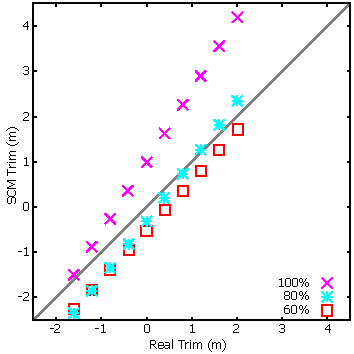
\includegraphics[scale=0.15]{figures/TrimScatter} & & 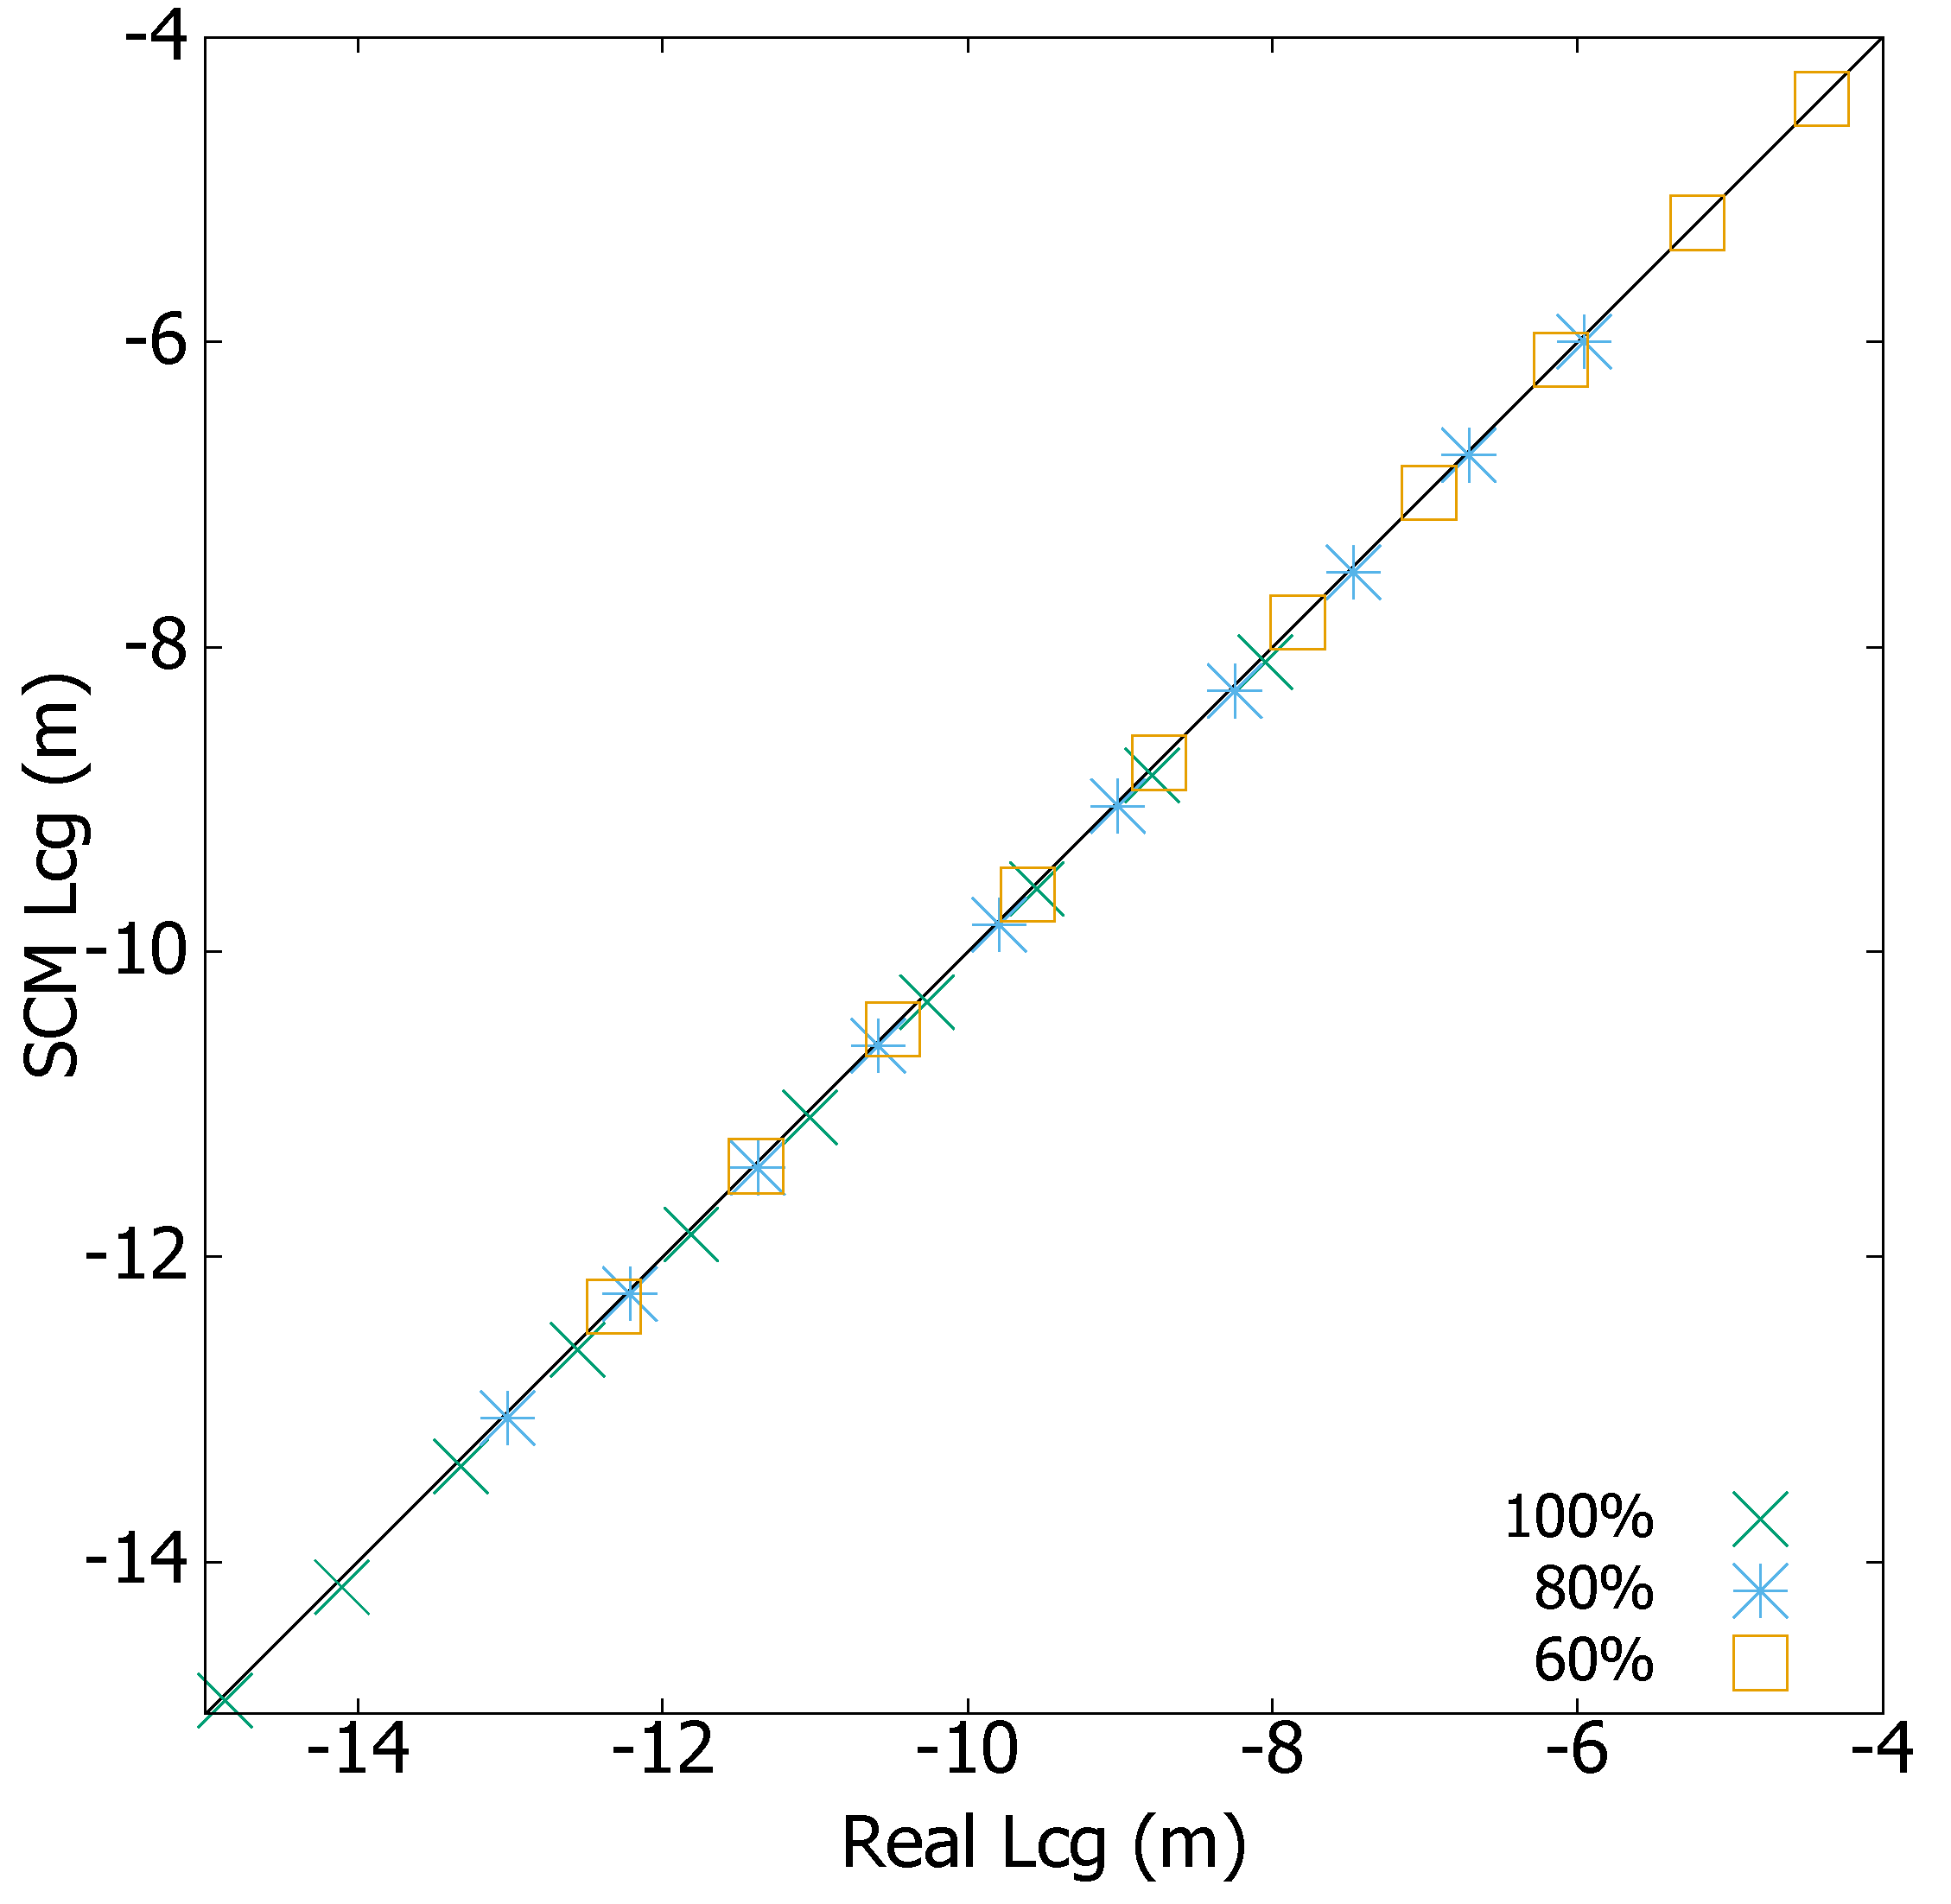
\includegraphics[scale=0.15]{figures/LcgScatter} \\
  (a) & \hspace{5mm} & (b)
\end{tabular}  
\end{center}
\caption{Correlations between real and predicted trim (a) and lcg (b) for a fixed partitioning with 26 sections and 60\%, 80\%, and 100\% of maximum displacement.}
\label{fig:trimlcgscatter}
\end{figure}
As depicted in the Fig.~\ref{fig:trimlcgscatter}(b) lcg is highly accurate for all weight distributions. We have that the longitudinal position of cargo weight is at the center of sections independently of the numbef of section. This, however, is not the case for lightship and tank blocks that usually are misaligned with section boundaries. What the results show is that impact on lcg at this level detail is negligible. The trim estimates shown in Fig.~\ref{fig:trimlcgscatter}(a) are very accurate for 80\% and 60\% of maximum displacement. Keep in mind that the vessel is almost 400 meters long, so the seen differences about 30 centimetres is an angular error of less than 0.1\%. That said, accurate trim estimates are highly valuable for the industry. We attribute the higher error at 100\% of maximum displacement to the underestimate of the buoyancy of the stern.
 
 
 
\subsection{Variable Section Partitioning for Fixed Displacement}

In the second set of experiments, we fix the displacement at 80\% of maximum  displacement, while the numbers of sections vary from 26 to 4. The trim and lcg predictions are shown in Table~\ref{tbl:trimVarPart} and \ref{tbl:lcgVarPart}, respectively.
\begin{table}[h!]
\begin{tabular}{rrr|rrrrrr}
\multicolumn{3}{c|}{Real Values}&\multicolumn{6}{c}{SCM Trim for Different}\\
\multicolumn{3}{c|}{}  &\multicolumn{6}{c}{Number of Sections}\\
Trim (m)       & Draft (m)   & Lcg (m)       & 26        &13        &10        &8          &6          &4\\
\hline
2.35        &13.11  &-13.02 & 2.01   &2.40    &2.54    &1.65    &0.78    &0.39\\
1.82        &13.13  &-12.21 &             1.61 &1.86           &2.02    &1.12    &0.24    &-0.16\\
1.27        &13.15  &-11.38 & 1.20 &1.31       &1.47    &0.57    &-0.30   &-0.68\\
0.73        &13.16  &-10.58 &             0.80 &0.79           &0.95    &0.00    &-0.88   &-1.20\\
0.20        &13.18  &-9.79   & 0.39 &0.26       &0.42    &-0.50   &-1.37   &-1.71\\
-0.32      &13.20  &-9.01   & 0.00 &-0.26     &-0.11   &-1.01   &-1.87   &-2.22\\
-0.82      &13.21  &-8.25   & -0.40 &-0.76   &-0.61   &-1.54   &-2.40   &-2.72\\
-1.34      &13.23  &-7.47   &             -0.80 &-1.28        &-1.12   &-2.03   &-2.93   &-3.20\\
-1.85      &13.25  &-6.71   &             -1.21 &-1.79        &-1.66   &-2.57   &-3.44   &-3.79\\
-2.35      &13.26  &-5.96   & -1.61 &-2.29   &-2.14   &-3.08   &-3.94   &-4.29\\
\end{tabular}
\caption{Trim predicted by SCM for 80\%of maximum displacement using six different partitionings.}
\label{tbl:trimVarPart}
\end{table}
\begin{table}
\begin{tabular}{rrr|rrrrrr}
\multicolumn{3}{c|}{Real Values}&\multicolumn{6}{c}{SCM Lcg for Different}\\
\multicolumn{3}{c|}{}&\multicolumn{6}{c}{Number of Sections}\\
Trim        & Draft   & Lcg       &26        &13        &10        &8          &6          &4\\
\hline
2.35        &13.11  &-13.02 &-13.06 &-13.12 &-13.21 &-11.88 &-11.14 &-11.09  \\
1.82        &13.13  &-12.21 &-12.25 &-12.33 &-12.42 &-11.09 &-10.31 &-10.23  \\
1.27        &13.15  &-11.38 &-11.42 &-11.49 &-11.61 &-10.27 &-9.48   &-9.43   \\
0.73        &13.16  &-10.58 &-10.62 &-10.72 &-10.84 &-9.43   &-8.59   &-8.63   \\
0.20        &13.18  &-9.79   &-9.82   &-9.91   &-10.05 &-8.68   &-7.84   &-7.85   \\
-0.32      &13.20  &-9.01   &-9.04   &-9.13   &-9.26   &-7.92   &-7.08   &-7.06   \\
-0.82      &13.21  &-8.25   &-8.29   &-8.38   &-8.51   &-7.13   &-6.28   &-6.28   \\
-1.34      &13.23  &-7.47   &-7.51   &-7.60   &-7.76   &-6.41   &-5.46   &-5.54   \\
-1.85      &13.25  &-6.71   &-6.74   &-6.83   &-6.95   &-5.60   &-4.69   &-4.64   \\
-2.35      &13.26  &-5.96   &-6.00   &-6.09   &-6.23   &-4.84   &-3.92   &-3.86   \\
\end{tabular}
\caption{Lcg predicted by SCM for 80\%of maximum displacement using six different partitionings.}
\label{tbl:lcgVarPart}
\end{table}
The correlations between the real trim and lcg and the predicted trim and lcg for these experiments are shown in Fig.~\ref{fig:trimLcgFixDisp}(a) and (b), respectively. As depicted Fig.~\ref{fig:trimLcgFixDisp}(b), the lcg positions depicted by SCM are systematically off for the coarser partitionings with 8, 6, and 4 sections with a fixed amount. This error may be due to the misalignment of lightship blocks and tanks which will be more significant at courser levels of the model. The the trim results shown Fig.~\ref{fig:trimLcgFixDisp}(a) are off correspondingly. 

It should be possible to factor out this off-set error 



\begin{figure}[h!]
\begin{center}
 \begin{tabular}{ccc}
  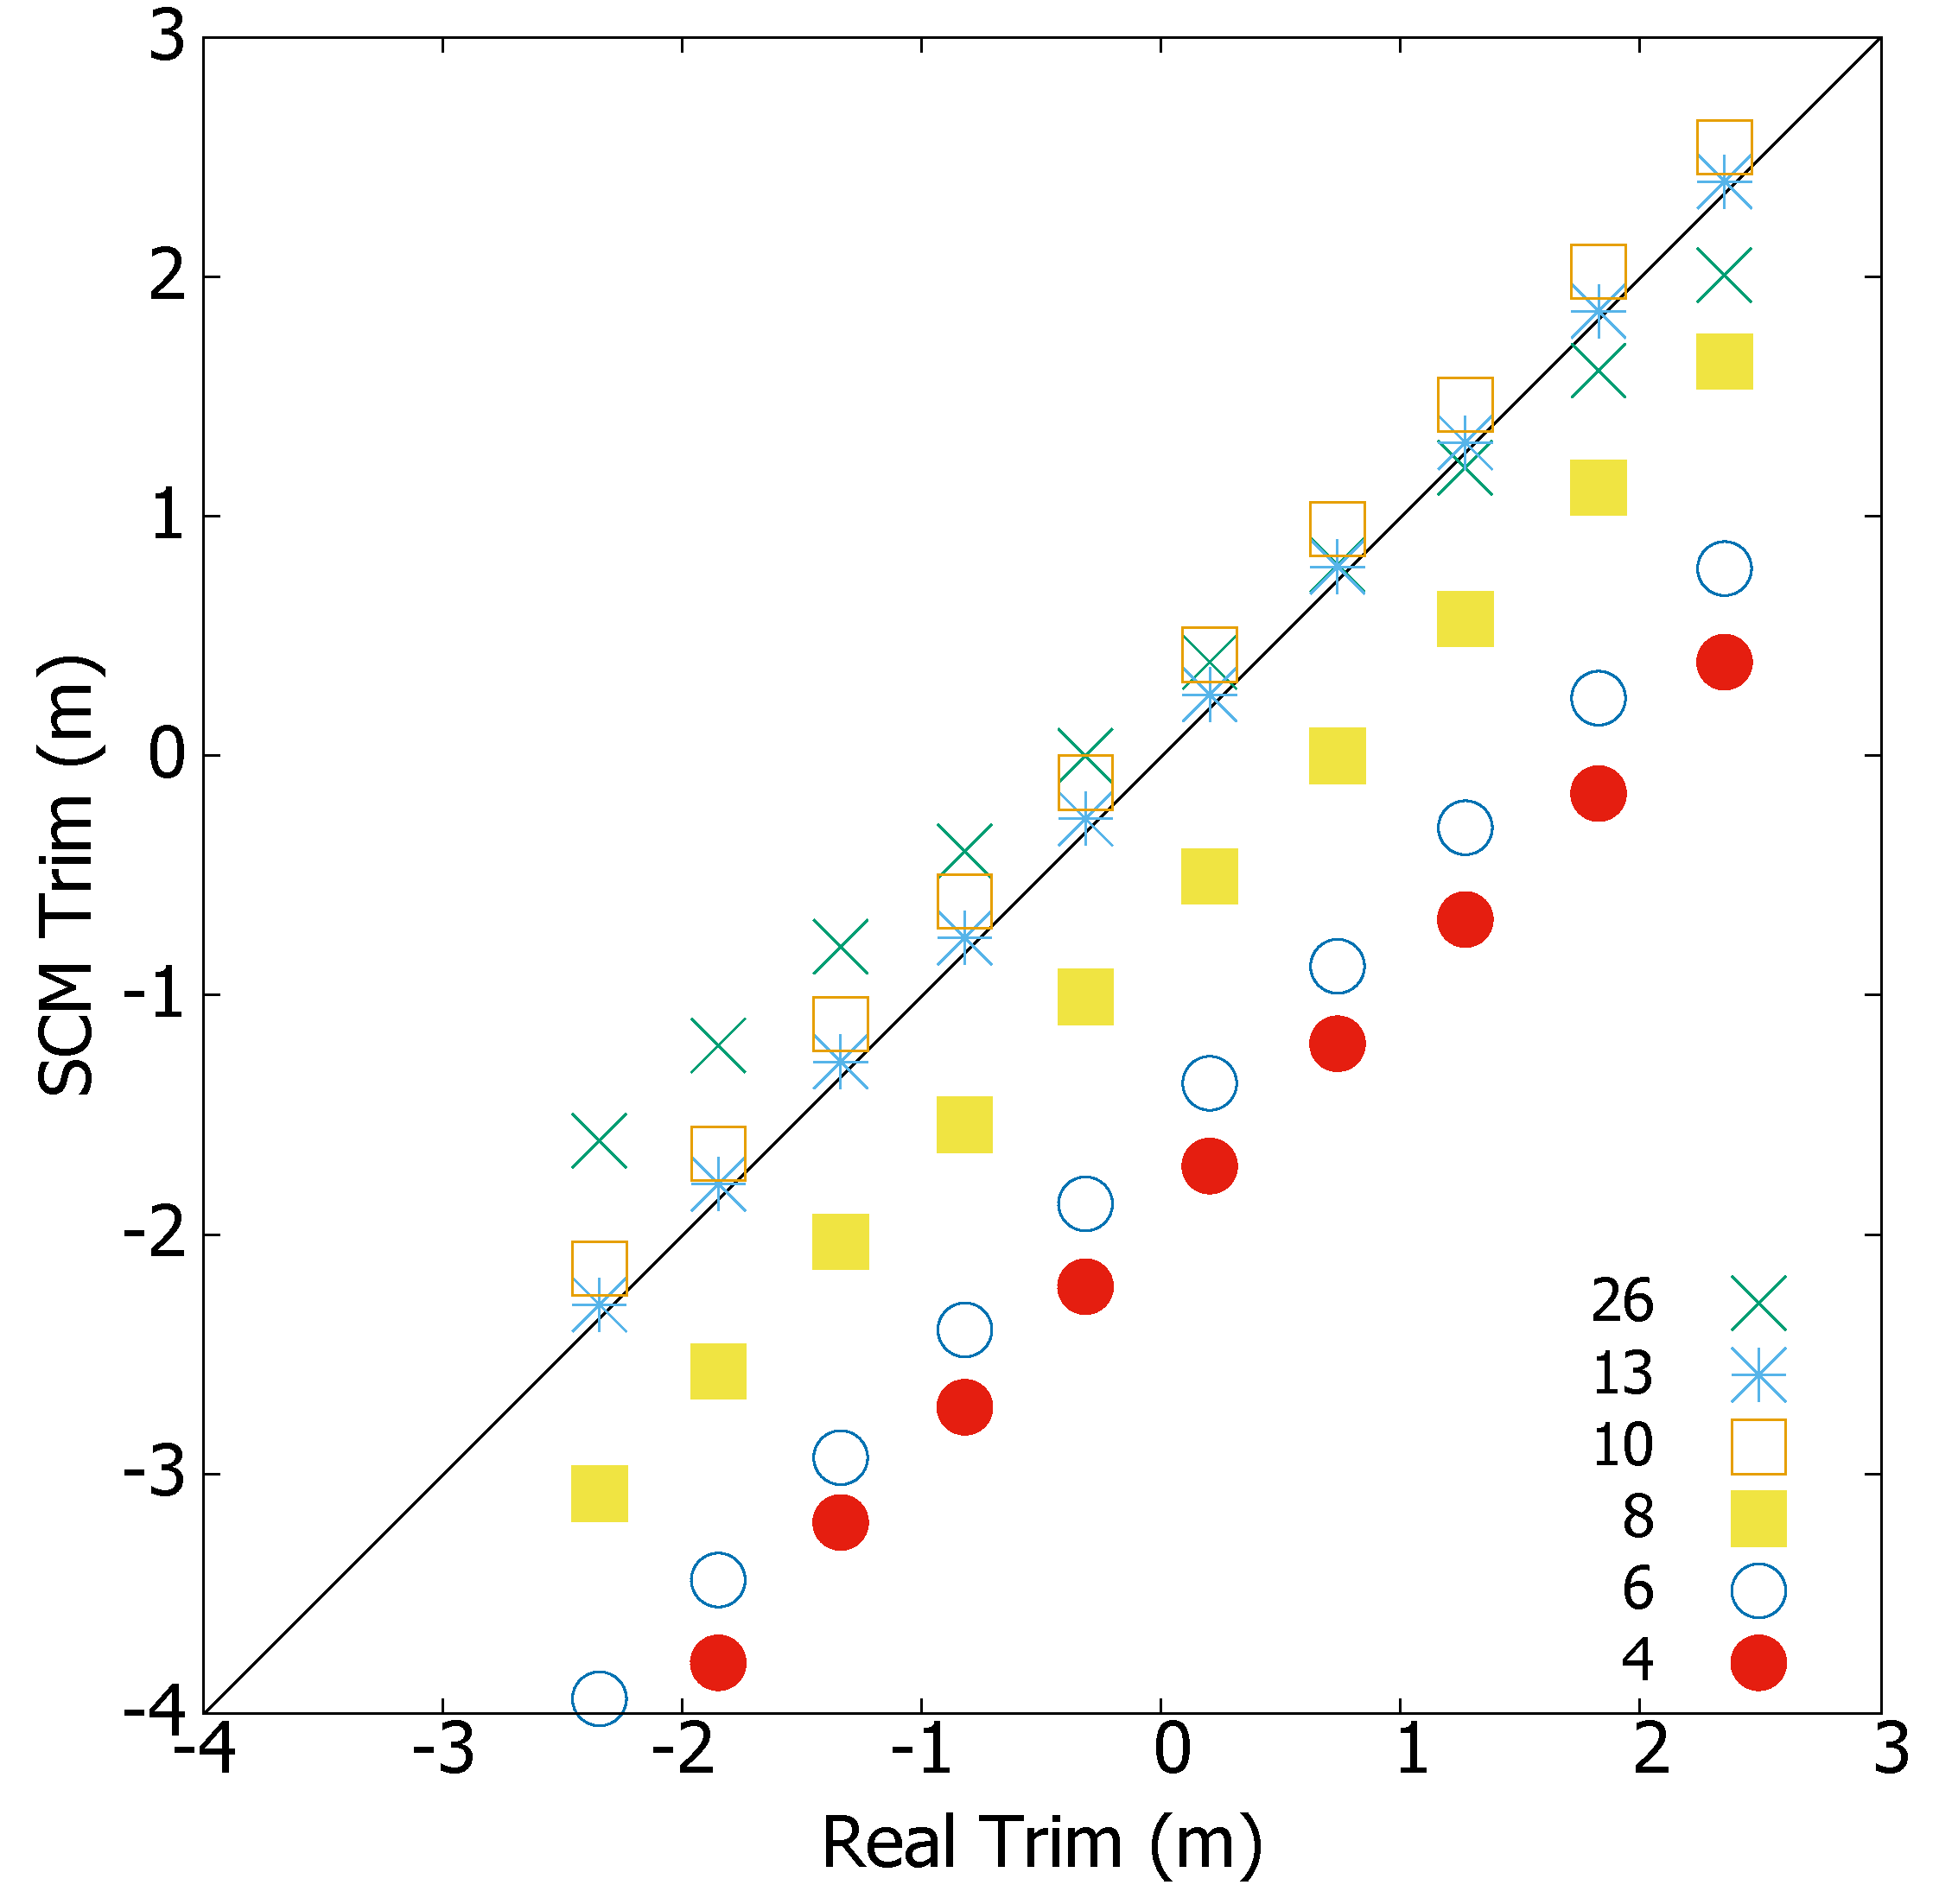
\includegraphics[scale=0.15]{figures/TrimVarSec} & & 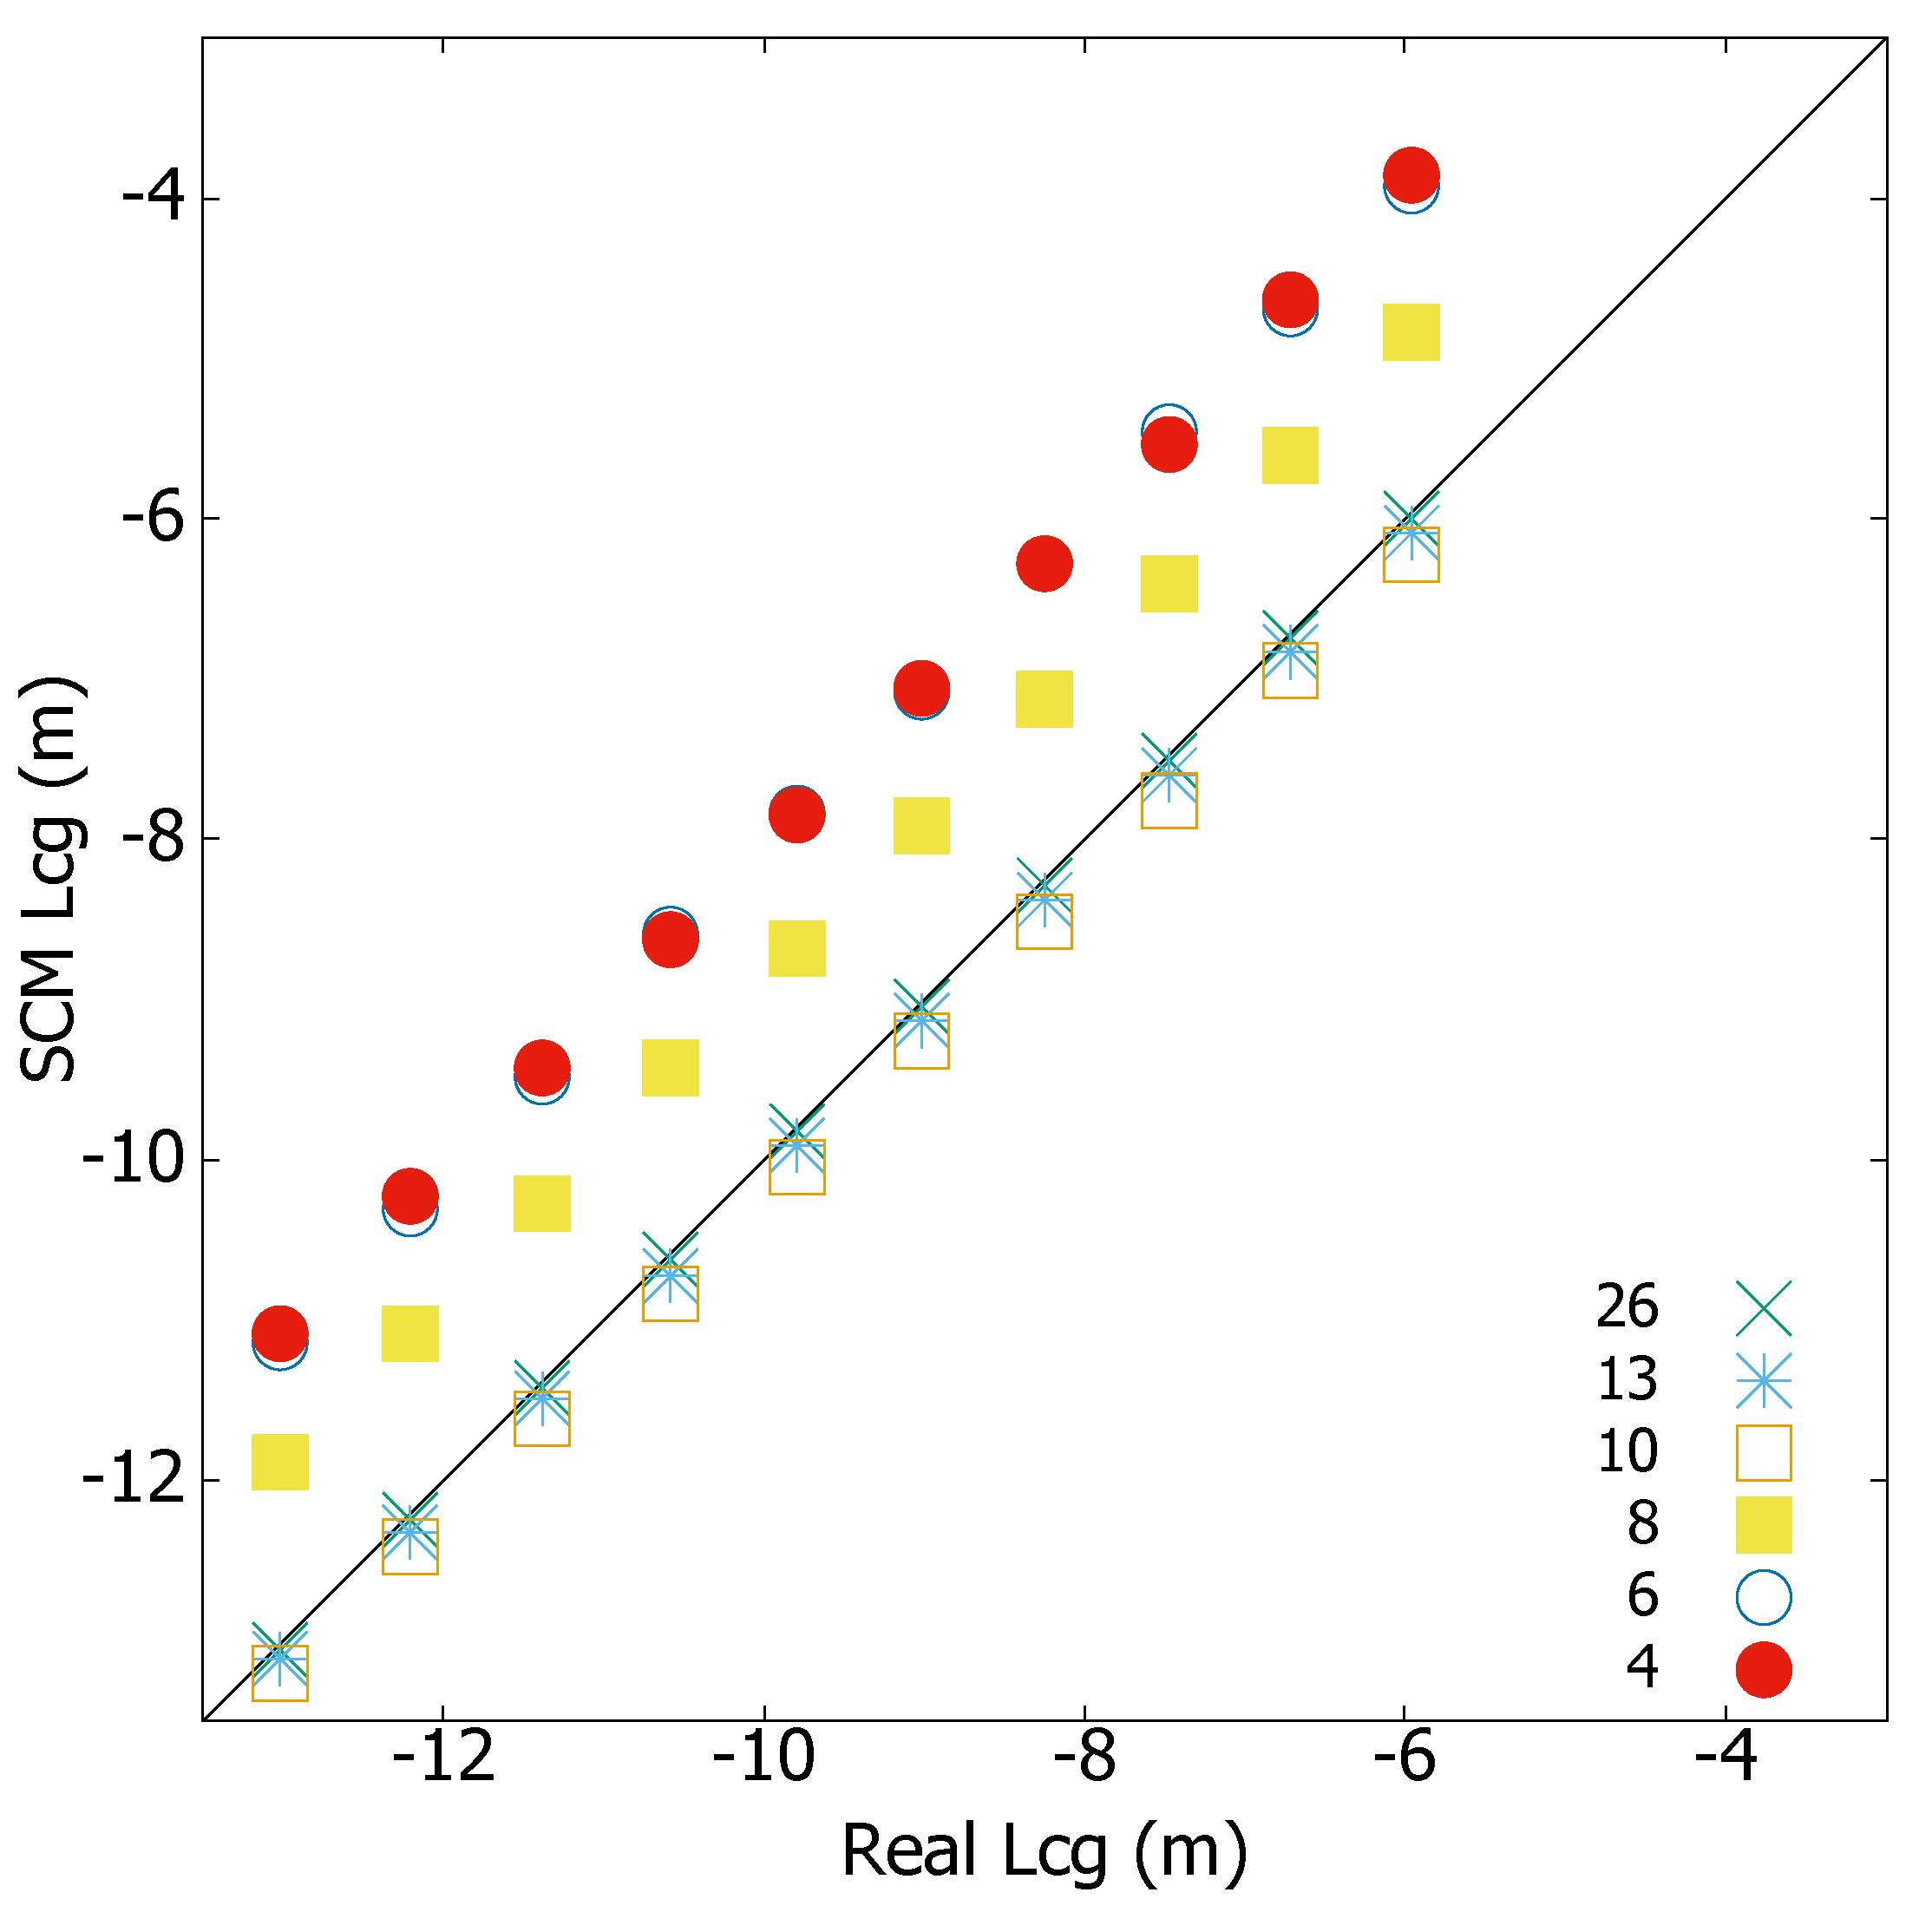
\includegraphics[scale=0.15]{figures/LcgVarSec} \\
  (a) & \hspace{5mm} & (b)
\end{tabular}  
\end{center}
\caption{Correlations between real and predicted trim (a) and lcg (b) for a fixed 80\% of maximum displacement and six different section partitionings.}
\label{fig:trimLcgFixDisp}
\end{figure}



 


\subsection{Stress Forces}
 
 
 
 \begin{figure}[h!]
\begin{center}
  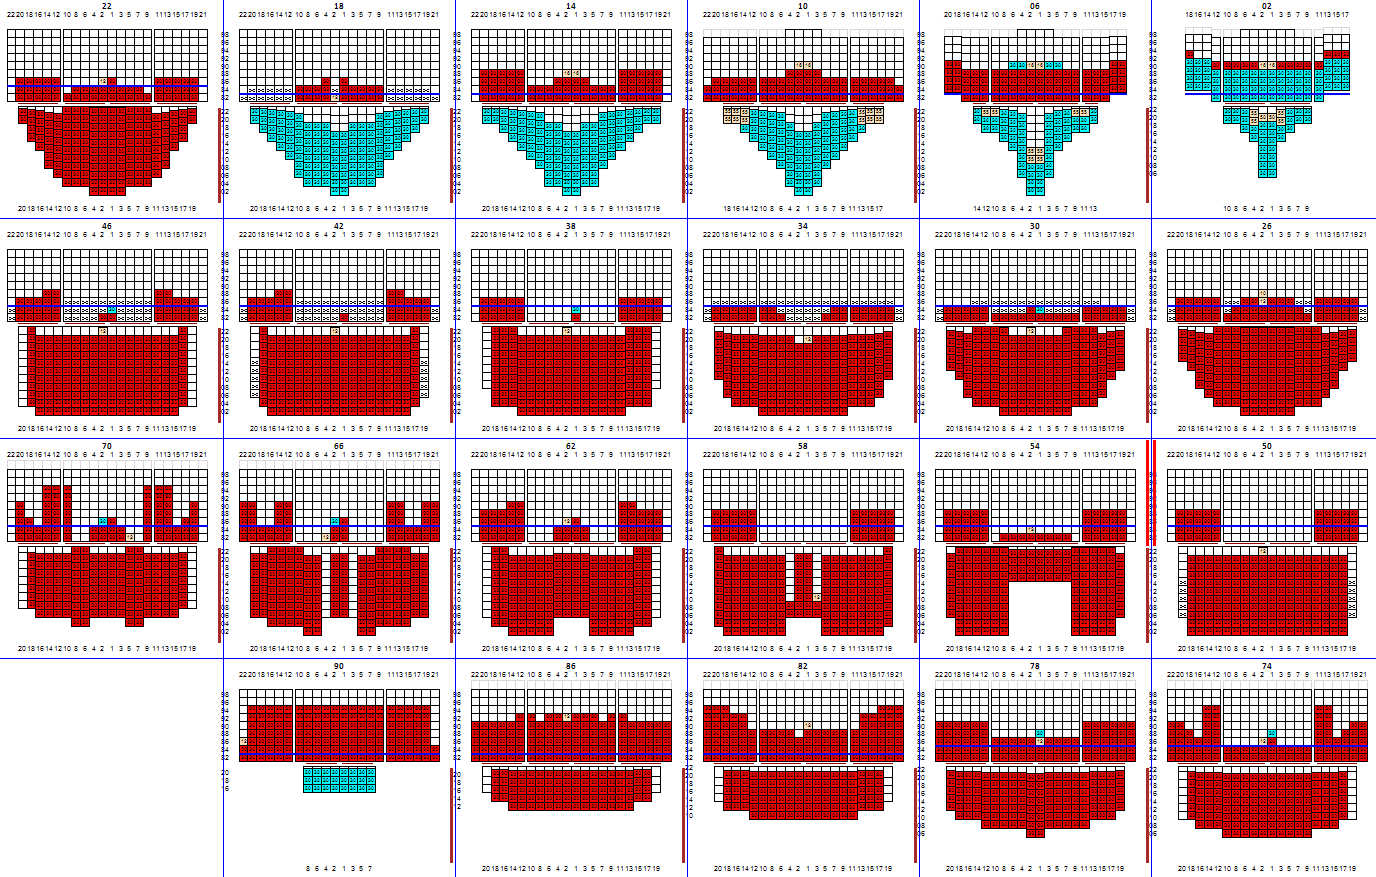
\includegraphics[scale=0.3]{figures/B31condition} 
\end{center}
\caption{Trim LCg Scatter}
\label{fig:trimlcgscatter}
\end{figure}

 
 
 
\begin{figure}[h!]
\begin{center}
 \begin{tabular}{ccc}
  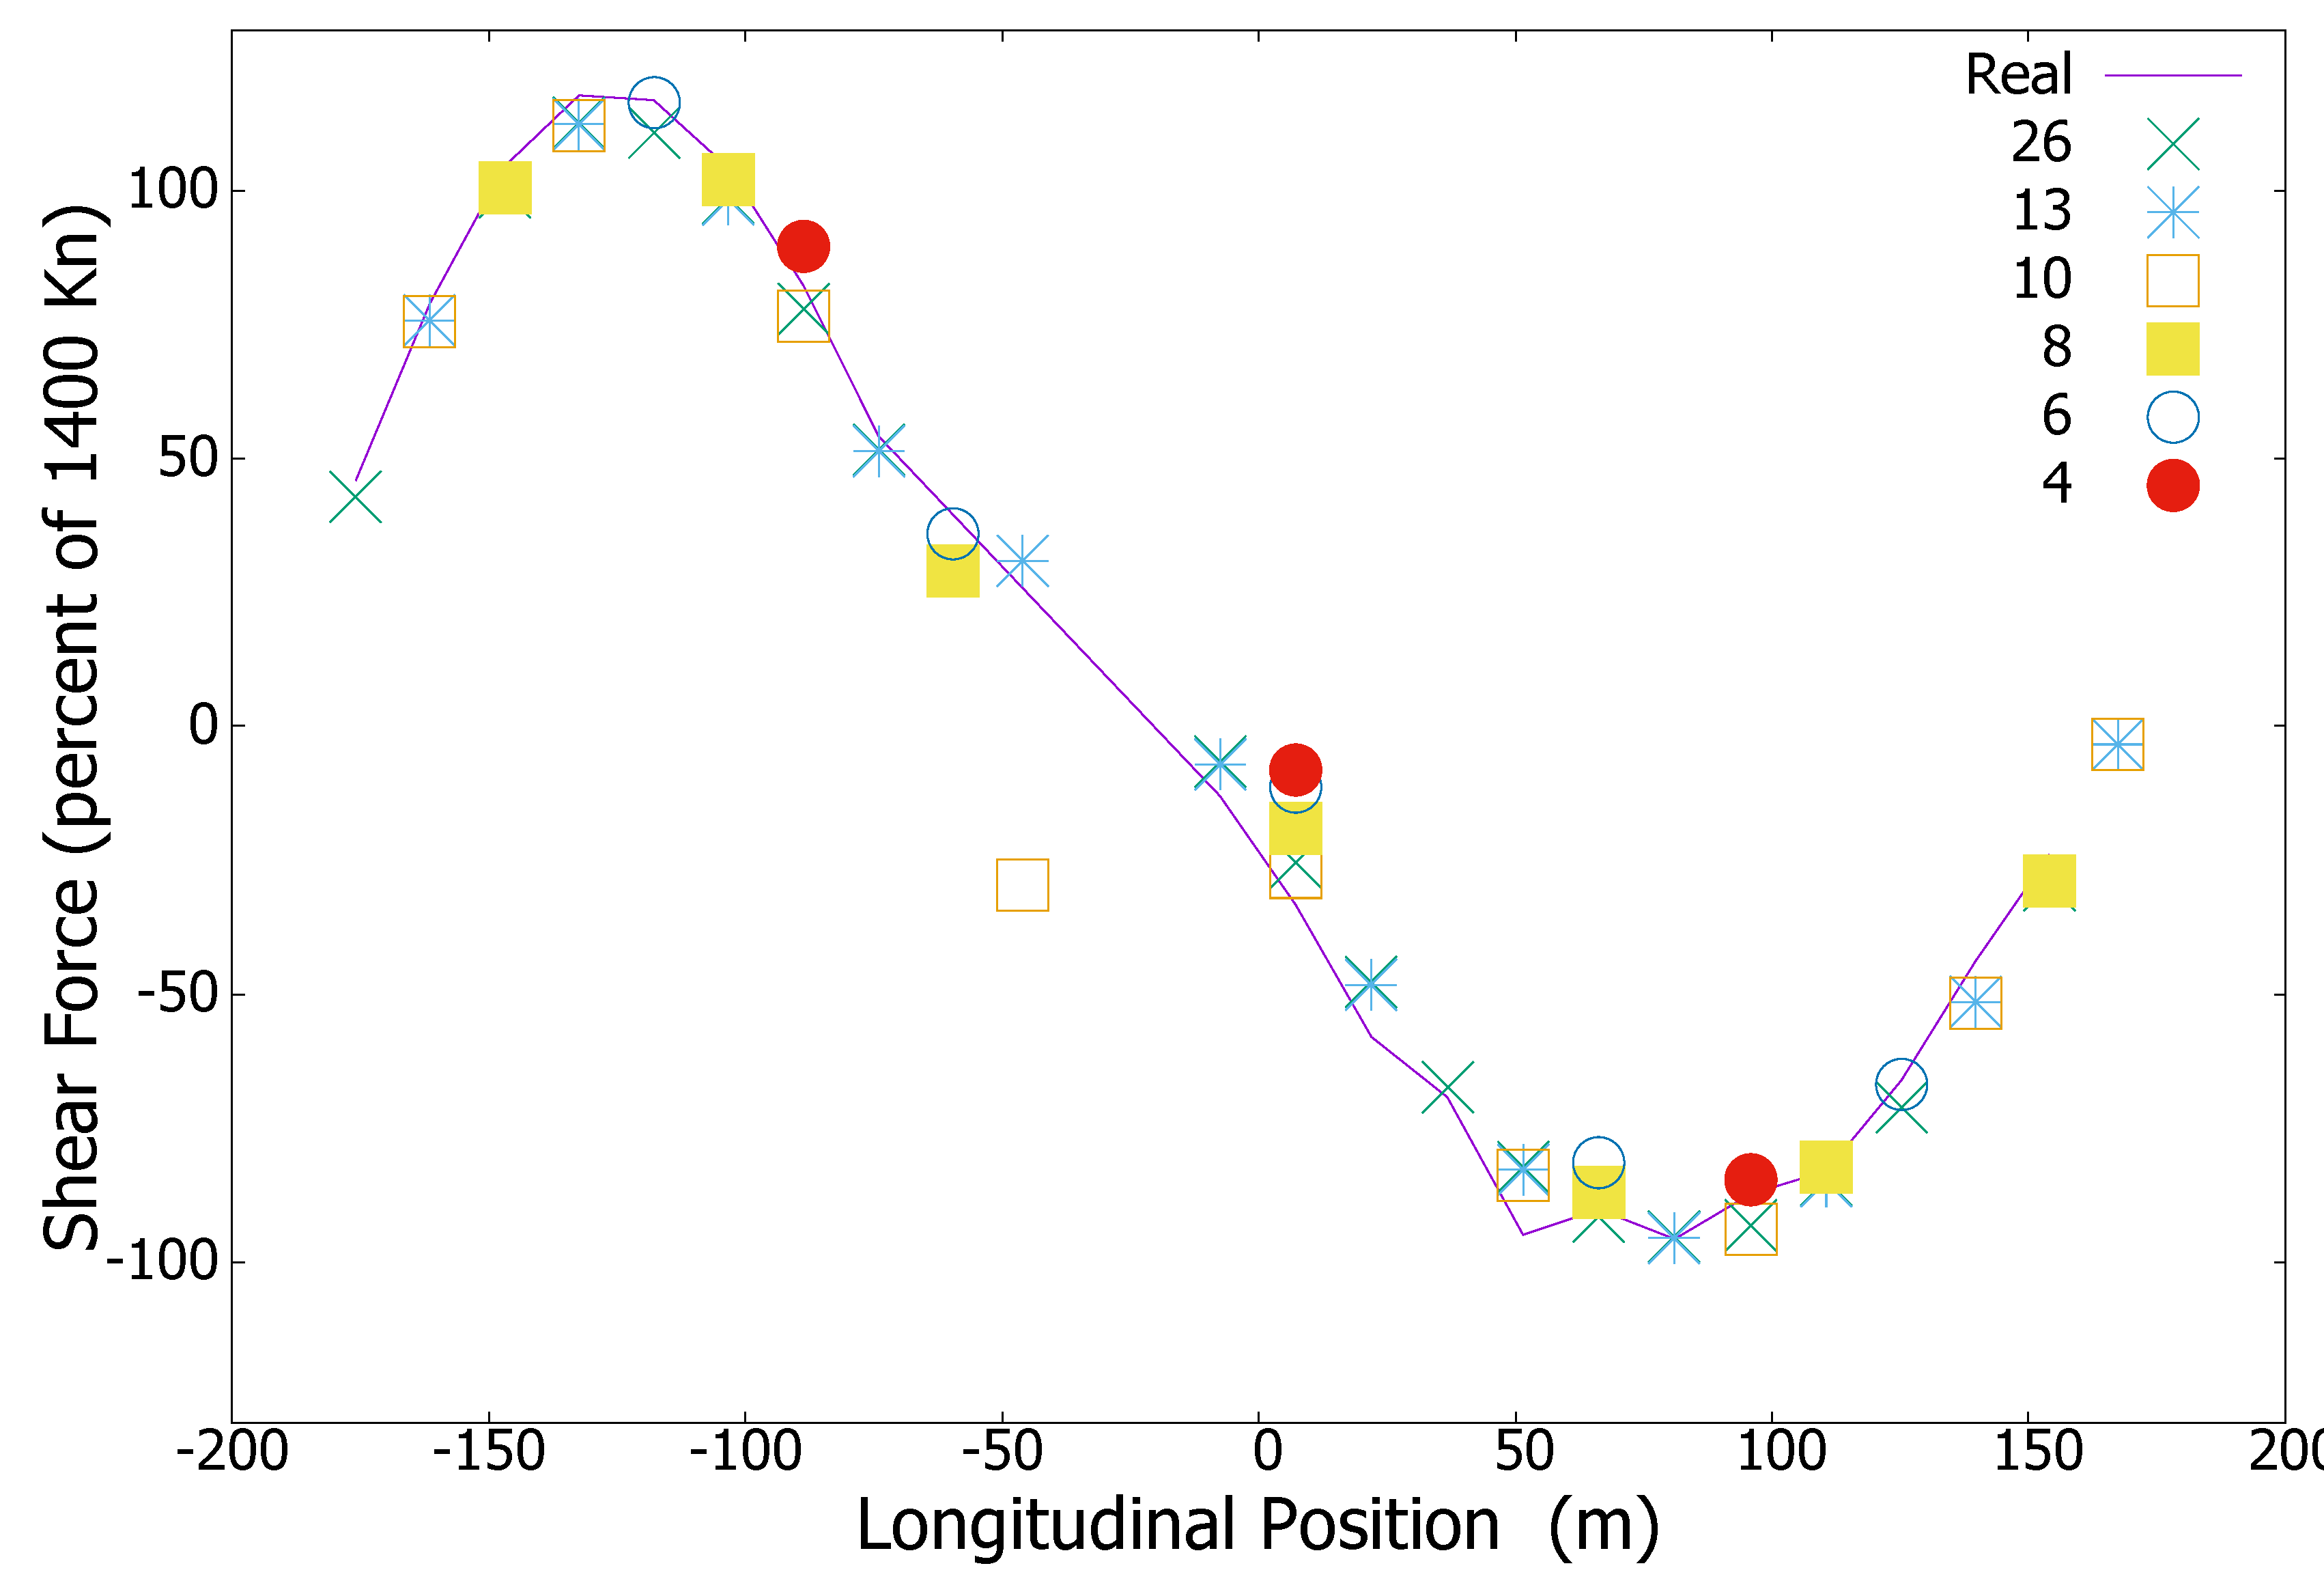
\includegraphics[scale=0.12]{figures/ShearForceplot} & & \includegraphics[scale=0.12]{figures/BendingMomentplot} \\
  (a) & \hspace{5mm} & (b)
\end{tabular}  
\end{center}
\caption{Trim LCg Scatter}
\label{fig:trimlcgscatter}
\end{figure}
 
 
 
 
 
\section{Conclusion and Future Work}

 In future work, we plan to extend the model with the advanced linear trade-off in stowage planning that we have found in our  industrial projects (cite E and K type).    

\bibliographystyle{splncs04}
\bibliography{references}

\end{document}
